\documentclass[conference]{IEEEtran}
\IEEEoverridecommandlockouts
\usepackage{quantikz}
% \usepackage{cite}
\usepackage[square,numbers]{natbib}
\usepackage{amsmath,amssymb,amsfonts}
\usepackage{algorithmic}
\usepackage{graphicx}
\usepackage{textcomp}
\usepackage{xcolor}
\usepackage{tikz}
\usepackage{braket}
\usepackage{bm}
\usepackage{hyperref}
\usepackage{booktabs}
\newcommand{\note}[1]{\textcolor{red}{[Note: #1]}}
\usepackage[colorinlistoftodos,prependcaption,textsize=tiny,textwidth=1cm,color=green]{todonotes}
\usepackage{subcaption}
\usepackage{tikz}
\usetikzlibrary{quantikz2}
\newsavebox{\DSCircuitBox}

\usepackage{amsthm}
\usepackage{mathtools}
 \usepackage{booktabs,threeparttable}
\newtheorem{theorem}{Theorem}
\newtheorem{lemma}[theorem]{Lemma}
\newtheorem{proposition}[theorem]{Proposition}
\newtheorem{corollary}[theorem]{Corollary}
\newtheorem{observation}[theorem]{Observation}

\newtheorem{assumption}[theorem]{Assumption}



\theoremstyle{definition}
\newtheorem{definition}[theorem]{Definition}
\newtheorem{hypothesis}[theorem]{Hypothesis}
\newtheorem{remark}[theorem]{Remark}
\newcommand{\xw}[1]{\textcolor{violet}{[XW: #1]}}
\definecolor{mlcolor}{RGB}{0,70,180}
\newcommand{\ml}[1]{\textcolor{mlcolor}{[ML: #1]}}
\usepackage{mathtools}

\usetikzlibrary{
    arrows.meta,
    backgrounds,
    calc,
    decorations.pathmorphing,
    fit,
    positioning
}

\DeclareMathOperator{\Tr}{Tr}
\DeclareMathOperator{\diag}{diag}

% Bell-correlation subspace and its Pauli--Liouville vector.
\newcommand{\SB}{\mathsf{S}_{\mathrm B}}
\newcommand{\plket}[1]{ \left. \left|#1\right\rangle \right \rangle_{\mathrm B}}

\usepackage{xspace}
\newcommand{\unicast}{{\normalfont \texttt{Unicast}}\xspace}
\newcommand{\mergecast}{{\normalfont \texttt{Mergecast}}\xspace}
\newcommand{\jce}{{\normalfont \texttt{JCE}}\xspace}
\newcommand{\mce}{{\normalfont \texttt{MCE}}\xspace}

\newcommand{\bellpair}[3]{%
    \draw[
        blue!70!black,
        line width=0.8pt,
        decorate,
        decoration={
            snake,
            amplitude=0.5mm,
            segment length=2.5mm
        }
    ] (#1,#2) -- (#1,#3);
    \filldraw[fill=white,draw=black,line width=0.8pt]
        (#1,#2) circle (2.2pt);
    \filldraw[fill=white,draw=black,line width=0.8pt]
        (#1,#3) circle (2.2pt);
}

\def\BibTeX{{\rm B\kern-.05em{\sc i\kern-.025em b}\kern-.08em
    T\kern-.1667em\lower.7ex\hbox{E}\kern-.125emX}}

\title{Freeriding Entanglement Distillation to Achieve Quantum Network Tomography}

% \author{...}

\begin{document}

\maketitle

\begin{abstract}




Entanglement distillation and quantum network tomography (QNT) address complementary needs in noisy quantum networks: the former improves the fidelity of distributed entanglement, while the latter identifies which internal links introduce the noise. Both require local measurement, yet they are typically treated as separate tasks. In this paper, we integrate QNT into end-to-end entanglement distillation by reusing the measurement statistics of the double-selection protocol, collected at peripheral monitors, for link-level characterization, so that distillation measurements come ``for free'' with respect to tomography. For a three-link star network with unknown Pauli channels, we combine Unicast and modified Mergecast preparations with Clifford dressing to identify all three Pauli channels. On this basis, we develop two estimators: the Joint-Coincidence Estimator (JCE), which exploits joint $X/Z$ coincidence statistics under a source-state fidelity condition $F > 1/2$, and the Marginal-Coincidence Estimator (MCE), which uses only Z-basis coincidence statistics with uniform Clifford dressing and removes this condition. We prove that both estimators uniquely identify all three Pauli channels without access to measurement outcomes at the central node. Qiskit simulations show that JCE and MCE recover channel parameters accurately while retaining fidelity-improved entangled pairs, and that retaining joint coincidence information improves estimation accuracy. We further extend JCE to a six-link triangular network, demonstrating applicability to more general network topologies beyond the star topology. These results demonstrate how distillation measurements can
support internal-link characterization without additional
measurements dedicated to tomography.111
\end{abstract}

\begin{IEEEkeywords}
Quantum Network Tomography, Entanglement Distillation, Mergecast.
\end{IEEEkeywords}

\section{Introduction}
\label{sec:introduction}

Distributing reliable entanglement across noisy quantum networks
is essential for secure communication, distributed quantum
computing, and networked quantum sensing
\cite{Wehner2018QuantumInternet}.
Shared entanglement enables quantum information processing
between distant nodes, but its usefulness is limited by noise
introduced during distribution.
Entanglement distillation and quantum network tomography (QNT)
address two complementary aspects of this problem.

Entanglement distillation uses local operations and classical
communication (LOCC) to probabilistically
 convert multiple noisy entangled pairs
into fewer pairs of higher fidelity   
\cite{PhysRevLett.76.722,Deutsch_1996}.
It provides a means to recover useful entanglement from imperfect
physical links and is an important component of quantum repeater
architectures \cite{Briegel1998Repeaters}.
For distributed quantum computing, improving shared entanglement
supports more reliable teleportation and quantum operations
between remote processors \cite{Wehner2018QuantumInternet}.

QNT infers the noise parameters of internal quantum links from
measurements performed at accessible peripheral nodes, termed
\emph{monitors} \cite{Andrade2024QNT}.
For experimental quantum networks, these estimates help diagnose
noisy links and guide distillation protocols.
For distributed quantum computing, they provide information for
predicting communication errors and selecting entanglement
distribution paths. The fidelity of an end-to-end state alone does not identify
which internal links introduce the noise; QNT seeks to recover
this link-level information from endpoint observations.
Together, entanglement distillation and QNT support
both the characterization and improvement of distributed quantum resources. Integrating them is particularly attractive when
generating entanglement is costly and measurement access is
restricted to peripheral nodes.

Despite their different objectives, entanglement distillation
and the QNT protocols considered here share a common operational feature: both rely on local measurements at accessible
nodes and classical processing of the outcomes. In distillation,
these outcomes determine whether an output pair is retained; in
QNT, their statistics are used to infer internal link parameters.
This operational similarity raises the possibility of using
distillation measurement statistics for network tomography









Casapao et al.\ pioneered the integration of entanglement
distillation and quantum state estimation with
Disti-Mator which
uses measurement statistics collected during entanglement
distillation to estimate the $X$-, $Y$-, and $Z$-basis parameters
that fully characterize a Bell-diagonal state under a fidelity
condition \cite{Casapao2025DistiMator}.
Their subsequent work developed a double-selection-based
estimator in \S~\ref{subsec:doub} using the marginal and joint coincidence statistics
collected during distillation \cite{Casapao_2025};
Motivated by these results, we identify a natural starting
point for QNT: the states shared by peripheral monitors
encode information about the individual links that we
use to distribute them.
We can therefore not only distill these states but also
estimate their parameters, and then use these estimates
to infer individual link parameters.
We thus integrate QNT into end-to-end distillation by using
distillation measurement statistics for link characterization
while also generating higher-fidelity entangled pairs,
thereby obtaining the best of both worlds.
We develop a Joint-Coincidence Estimator (JCE) and a
Marginal-Coincidence Estimator (MCE) for this task.




Realizing this idea requires overcoming two challenges. First,
state estimation does not automatically imply link identifiability.
In a three-link star network with Pauli channels, direct Unicast
transmission yields pairwise products of link-level Pauli transfer
matrix (PTM) eigenvalues. From these products, one can estimate the absolute value of the link parameters but with a sign ambiguity. To resolve this ambiguity, we adapt the Mergecast
and channel-dressing techniques introduced
in \cite{wang2025quantumnetworktomographygeneral} to prepare
Bell-diagonal states for double-selection measurements.
Mergecast provides estimates of three-link correlations,
while Clifford dressing makes the required Pauli components
accessible. Combining these estimates with those of the pairwise
products enables estimation of both the magnitudes and
signs of the link parameters without access to measurement
outcomes from the central node.

Second, inherited from the double-selection protocol, estimating all three state parameters \(q_X, q_Y, q_Z\) requires a source-state fidelity condition, implying another sign ambiguity of the protocol itself.
 This condition restricts
the noise regimes in which JCE applies. We overcome this
restriction in MCE  by observing that
the $Z$-basis parameter can be uniquely recovered without
a fidelity condition. Applying uniform Clifford dressings
maps the original $X$ and $Y$ components to the effective
$Z$ component. Repeating the estimation in these configurations
therefore enables the estimation of all link parameters
without the source-state fidelity requirement.

Our contributions are summarized as follows:
\begin{itemize}
    \item In \S~\ref{sec:dist-qnt}, we develop a distillation-assisted QNT framework for a
    three-link star network with unknown Pauli channels. The framework
    integrates Unicast and adapted Mergecast preparations with
    double-selection measurements at peripheral monitors, using
    measurement statistics from both accepted and rejected attempts for estimation.
    The central node performs prescribed operations without supplying
    measurement outcomes to the tomography procedure.

\item In \S~\ref{linkpa}, we construct two estimators to identify
the parameters of each Pauli channel in the three-link star network.
JCE combines estimates of pairwise and three-link correlations
with link-dependent Clifford dressing under the specified
source-state fidelity condition $F>1/2$.
MCE combines $Z$-basis coincidence statistics with uniform
Clifford dressing and requires no source-state fidelity condition.
\textcolor{blue}{
\item In \S~\ref{sec:numerical-experiments}, we evaluate JCE and MCE through
Qiskit simulations and compare their estimation accuracy
with existing QNT methods under different measurement
budgets and prior assumptions. The results demonstrate
the benefit of joint coincidence statistics for estimation
and show that both estimators can recover channel parameters
while retaining entangled pairs with improved fidelity.
We further extend JCE to a six-link triangular network,
demonstrating its applicability beyond the three-link
star topology.
```}

\end{itemize}

% \subsection{Related Work}
% Entanglement distillation has developed from foundational two-party
% protocols into a key tool for long-distance quantum communication.
% In 1996, Bennett et al.\ established a distillation protocol for
% extracting high-quality entangled pairs from noisy shared states
% \cite{PhysRevLett.76.722}, while Deutsch et al.\ introduced a
% purification-based quantum privacy amplification protocol
% \cite{Deutsch_1996}. Briegel et al.\ subsequently incorporated nested
% purification into quantum repeaters, connecting local entanglement
% processing with entanglement distribution over long distances
% \cite{Briegel1998Repeaters}. Further developments addressed the
% effects of imperfect local operations. In particular, Fujii and
% Yamamoto introduced double selection, which uses two ancillary pairs
% to improve error detection and achieve higher purification fidelities
% and noise thresholds than single selection in the regimes they
% studied \cite{PhysRevA.80.042308}.

% The development of QNT has focused on recovering internal link
% properties despite limited measurement access. In 2022, de Andrade
% et al.\ formulated end-to-end channel characterization through
% multipartite state distribution and studied star networks with
% single-Pauli noise, including bit-flip channels
% \cite{Andrade2022MultipartiteQNT}. Subsequent work developed
% protocols for uniquely characterizing quantum flip stars and used
% quantum Fisher information to compare their estimation performance
% \cite{Andrade2023FlipStars}. The framework was also applied to
% depolarizing channels, extending its scope beyond bit-flip noise
% \cite{Andrade2024QNT}. More recently, Wang et al.\ introduced
% Mergecast and a progressive etching procedure to address
% identifiability in networks with general Pauli channels and broader
% topologies, and further considered state-preparation and measurement
% (SPAM) errors \cite{wang2025quantumnetworktomographygeneral}.
% These studies establish methods for extracting link information
% from network-level observations, motivating the use of other
% network operations as sources of tomographic data.

\section{Preliminaries}

\subsection{Pauli--Liouville Representation}

To facilitate the analysis of distillation, we present the Pauli--Liouville representation \cite{Lin2021} in the two-qubit scenario below.
Let
\(
\mathbb{P}_2 \coloneqq\{I,X,Y,Z\}^{ \otimes 2}
\)
denote the two-qubit Pauli operator basis, which is a
complete orthogonal basis for the operator space
$\mathcal{L}\bigl((\mathbb{C}^{2})^{\otimes 2}\bigr)$ under the
Hilbert--Schmidt inner product. Then, every two-qubit operator $\mathcal{G}$ can be uniquely expressed as a linear combination of the elements of $\mathbb P_2$.
% admits a unique Pauli
% expansion as a linear combination of the Pauli basis elements.
Define the Pauli coefficient associated with
$P\in\mathbb{P}_2$ as
\begin{equation}
        s_P(\mathcal G)\coloneqq\operatorname{Tr}\!\left(P^{\dagger}\mathcal{G}\right),
\end{equation}
we can express $\mathcal{G}$ as follows,
\begin{equation}
    \mathcal{G}=\frac{1}{4}\sum_{P\in\mathbb{P}_2}s_P(\mathcal{G})P.
    \label{eq:pauli-expansion}
\end{equation}

Following the Pauli-Liouville representation,
we introduce the \(\left|\cdot\right\rangle\!\rangle\)  notation, and with it, the state can be expressed as a column vector as follows:
\begin{equation}
    \begin{aligned}
        \left|\rho\right\rangle\!\rangle
        \coloneqq\bigl[s_P(\rho)\bigr]^T_{P\in\mathbb{P}_2}.
    \end{aligned}
    \label{eq:pauli-liouville-vectors}
\end{equation}

For a two-qubit linear map \(\mathcal E\), its Pauli transfer matrix (PTM) \(R_{\mathcal E}\) is a \(16\times16\) matrix, whose enties are
\begin{equation}
    \left(R_{\mathcal E}\right)_{P,Q}
    \coloneqq\frac{1}{4}\Tr\!\left[P^\dagger\mathcal E(Q)\right],
    \text{ for any } P,Q\in\mathbb{P}_2.
    \label{eq:ptm-definition}
\end{equation}
Consequently, the outcome state of applying the operator \(\mathcal E\) to an input state \(\rho\) can be expressed as follows,
\begin{equation}
    \begin{aligned}
        \left|\mathcal E(\rho)\right\rangle\!\rangle
         & =R_{\mathcal E}\left|\rho\right\rangle\!\rangle.
    \end{aligned}
    \label{eq:pauli-liouville-born-rule}
\end{equation}


\subsection{Pauli Channels in Bell-Diagonal Basis}

% Bell states are particularly convenient for describing two-qubit
% entanglement under Pauli noise because single-qubit Pauli errors
% permute the Bell states. 
Bell basis (composed by Bell states) is particularly convenient for describing two-qubit
entanglement under Pauli noise because applying a single-qubit Pauli error to one half of a Bell pair maps it to another Bell state.
The four Bell states are
\begin{equation}
    \ket{\Phi^\pm}
    =
    \frac{\ket{00}\pm\ket{11}}{\sqrt{2}},
    \qquad
    \ket{\Psi^\pm}
    =
    \frac{\ket{01}\pm\ket{10}}{\sqrt{2}}.
\end{equation}

Their density operators admit the Pauli decomposition
\begin{equation}
    \begin{aligned}
        \ket{\Phi^+}\!\bra{\Phi^+}
         & =
        \frac{1}{4}
        \left(
        I I
        +X X
        -Y Y
        +Z Z
        \right), \\
        \ket{\Psi^+}\!\bra{\Psi^+}
         & =
        \frac{1}{4}
        \left(
        I I
        +X X
        +Y Y
        -Z Z
        \right), \\
        \ket{\Psi^-}\!\bra{\Psi^-}
         & =
        \frac{1}{4}
        \left(
        I I
        -X X
        -Y Y
        -Z Z
        \right), \\
        \ket{\Phi^-}\!\bra{\Phi^-}
         & =
        \frac{1}{4}
        \left(
        I I
        -X X
        +Y Y
        +Z Z
        \right).
    \end{aligned}
    \label{eq:bell-projector-pauli-expansions}
\end{equation}

These decompositions motivate the definition of the operator subspace
\begin{equation}
    \mathcal S_{\mathrm B}
    \coloneqq
    \operatorname{span}
    \{I I, X X, Y Y, Z Z\}.
    \label{eq:bell-diagonal-subspace}
\end{equation}
An operator belongs to $\mathcal S_{\mathrm B}$ if it is a linear
combination of these four Pauli operators.

A two-qubit density operator $\rho$ is called Bell-diagonal if it
is diagonal in the Bell basis. By
Lemma~\ref{lem:bell-pauli-transformation}, this is equivalent to
$\rho\in\mathcal S_{\mathrm B}$.

For such a state, we define its restricted Pauli--Liouville vector as
\begin{equation}
    \plket{\rho}
    \coloneqq
    \begin{bmatrix}
        s_{II}(\rho)  &
        s_{XX}(\rho)  &
        s_{Y Y}(\rho) &
        s_{Z Z}(\rho)
    \end{bmatrix}^{ T},
    \label{eq:restricted-pauli-liouville-vector}
\end{equation}
where $s_P(\rho)\coloneqq\operatorname{Tr}(P^\dagger\rho)$.

The relation between the Bell basis and the Pauli basis is
standard~\cite{Horodecki1996,Luo2008}. For completeness of presentation, we state the
corresponding change-of-basis relation below.

\begin{lemma}
    \label{lem:bell-pauli-transformation}
    Consider the following ordered bases of \(\mathcal S_B\):
    \begin{equation}
        \begin{aligned}
            \mathcal B_{\mathrm{Bell}}
             & \coloneqq
            \left(
            \ket{\Phi^+}\!\bra{\Phi^+},
            \ket{\Psi^+}\!\bra{\Psi^+},
            \ket{\Psi^-}\!\bra{\Psi^-},
            \ket{\Phi^-}\!\bra{\Phi^-}
            \right),     \\
            \mathcal B_{\mathrm P}
             & \coloneqq
            \left(
            I I,
            X X,
            Y Y,
            Z Z
            \right).
        \end{aligned}
        \label{1}
    \end{equation}
    There exists a full-rank transformation matrix $W$ which satisfies $4WW^T= I_4$ such that
    \begin{equation}
        \mathcal{B}_{\mathrm{Bell}}
        =
        \mathcal{B}_{\mathrm{P}}W,
        \qquad
        W=
        \frac{1}{4}     \begin{bmatrix*}[r]
         1 &  1 &  1 &  1 \\
         1 &  1 & -1 & -1 \\
        -1 &  1 & -1 &  1 \\
         1 & -1 & -1 &  1
    \end{bmatrix*}.
        \label{eq:bell-pauli-transform}
    \end{equation}
\end{lemma}

For a normalized state \(\rho\), its fidelity is defined as
\begin{equation}
    \begin{aligned}
        F(\rho)
         & =\frac{1}{4}\left[
                           s_{I I}(\rho)
                           +s_{X X}(\rho)
                           -s_{Y Y}(\rho)
                           +s_{Z Z}(\rho)
                           \right].
    \end{aligned}
    \label{eq:bell-state-fidelity}
\end{equation}

Consider the single-qubit Pauli channel
\begin{equation}
    \mathcal P(\sigma)
    =
    A\sigma
    +BX\sigma X
    +CY\sigma Y
    +DZ\sigma Z,
    \label{eq:single-qubit-pauli-channel}
\end{equation}
where
\(
A, B, C, D\geq 0
\) and \(
A+B+C+D=1.
\)
If the first qubit is unaffected and the second qubit undergoes
\(\mathcal P\), the corresponding two-qubit channel is
\(
\mathcal E=\mathcal I\otimes\mathcal P,
\)
where \(\mathcal I\) denotes the identity channel.
Applying this channel to the maximally entangled state
\(\ket{\Phi^+}\) produces the Bell-diagonal state
\begin{equation}
    \begin{aligned}
        \rho
         & =
        \mathcal E\left(\ket{\Phi^+}\!\bra{\Phi^+}\right) \\
         & =
        A\ket{\Phi^+}\!\bra{\Phi^+}
                       {+}B\ket{\Psi^+}\!\bra{\Psi^+}
                                         {+}C\ket{\Psi^-}\!\bra{\Psi^-}
                                                           {+}D\ket{\Phi^-}\!\bra{\Phi^-}.
    \end{aligned}
    \label{eq:pauli-channel-output-state}
\end{equation}


As defined in \eqref{eq:ptm-definition}, the full PTM
\(R_{\mathcal E}\) is a \(16\times16\) matrix with respect to the
complete two-qubit Pauli basis. However, $\mathcal S_{\mathrm B}$ is invariant under $\mathcal E$,
meaning that $\mathcal E(\mathcal{G})\in\mathcal S_{\mathrm B}$ for every
$\mathcal{G}\in\mathcal S_{\mathrm B}$. Therefore, the action of \(\mathcal E\) on
Bell-diagonal states is completely described by its restriction to
\(\mathcal S_B\). With respect to the ordered basis
\(\mathcal B_{\mathrm P}\) in \ref{1}, the resulting \(4\times4\) PTM is
\begin{equation}
    \begin{aligned}
        \left.R_{\mathcal E}\right|_{\mathcal S_B}
         & =
        \operatorname{diag}(1,q_X,q_Y,q_Z), \\
        q_X
         & =
        A+B-C-D
        =
        2(A+B)-1,                           \\
        q_Y
         & =
        A-B+C-D
        =
        2(A+C)-1,                           \\
        q_Z
         & =
        A-B-C+D
        =
        2(A+D)-1.
    \end{aligned}
    \label{eq:pauli-channel-ptm}
\end{equation}
Here, \(q_X,q_Y,q_Z\) are also the eigenvalues of the single-qubit
Pauli channel on \(X,Y,Z\), respectively. It is obvious that $q_X,q_Y,q_Z\in [-1,1],
$
which leads to the identification challenge in QNT, we will elaborate this later in \S \ref{subsec:direct-nt}.

Consequently, the output state in
\eqref{eq:pauli-channel-output-state} has the Pauli decomposition
\begin{equation}
    \rho
    =
    \frac{1}{4}
    \left(
    I I
    +q_X X X
    -q_Y Y Y
    +q_Z Z Z
    \right),
    \label{eq:pauli-channel-output-expansion}
\end{equation}
and its restricted Pauli--Liouville vector is
\begin{equation}
    \plket{\rho}
    =
    \begin{bmatrix}
        1 & q_X & -q_Y & q_Z
    \end{bmatrix}^{T}.
    \label{eq:pauli-channel-output-vector}
\end{equation}


By Lemma~\ref{lem:bell-pauli-transformation}, the Pauli coefficients
of state $\rho$ uniquely determine the channel parameters
\(A,B,C,D\).


\subsection{Double-Selection Protocol}
\label{doub}\label{subsec:doub}

Entanglement distillation aims to  probabilistically
 transform multiple copies of a noisy
entangled pairs into  fewer pairs with higher fidelity to a target Bell
state, which we take to be $\ket{\Phi^+}$.
For example, the protocol considered here uses two noisy ancillary
pairs to probabilistically increase the fidelity of a third pair.
Recent work has shown that measurement statistics collected during
entanglement distillation can also be used for state
estimation~\cite{Casapao_2025}.

We consider the double-selection protocol introduced by Fujii and
Yamamoto~\cite{PhysRevA.80.042308}.
Figure~\ref{fig:double-selection-circuit} illustrates its dual role:
successful attempts yield purified entangled pairs, while measurement
records from all attempts are used to estimate the input
Bell-diagonal state under the conditions specified below.


\begin{figure*}[tb]
    \centering
    \resizebox{\textwidth}{!}{%
        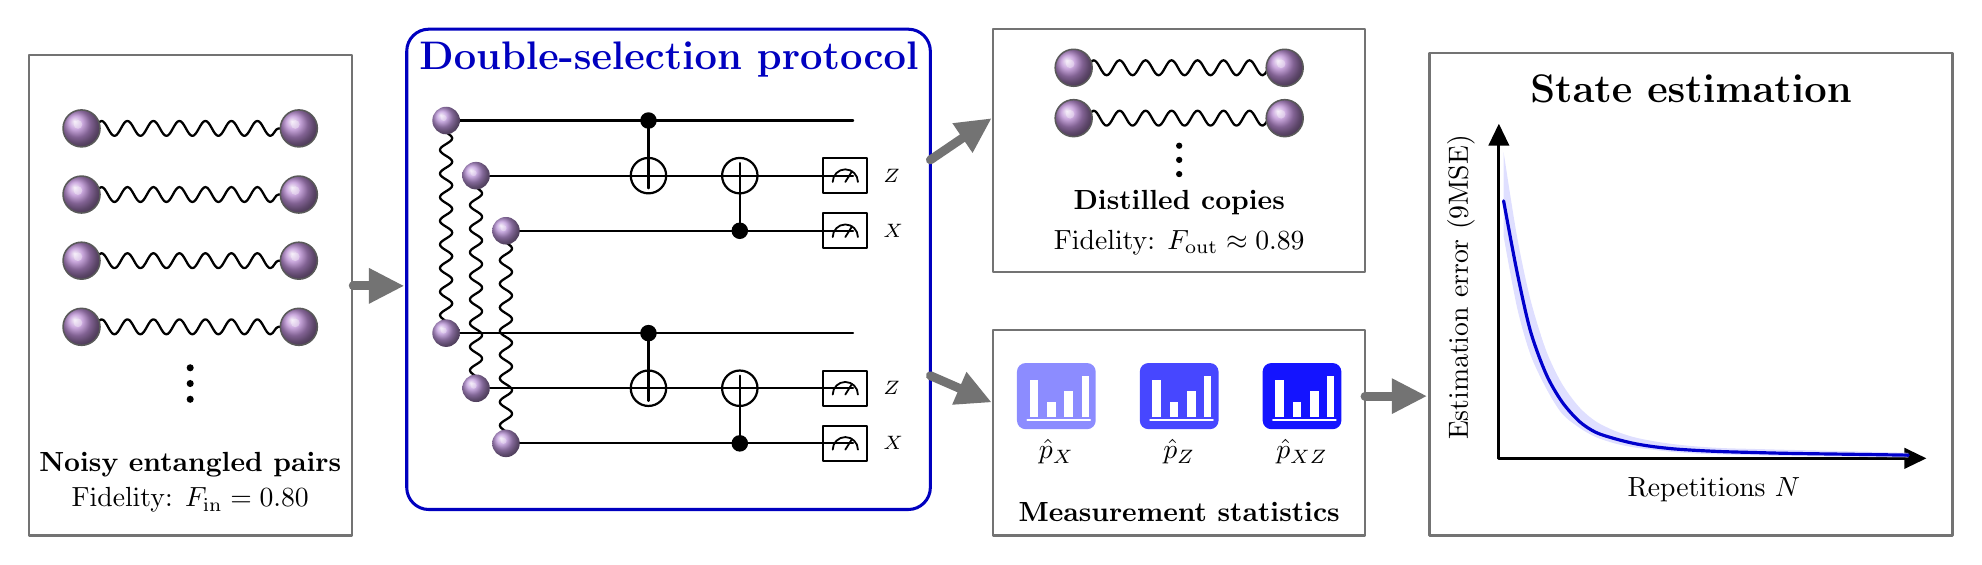
\begin{tikzpicture}[x=1cm,y=1cm,line cap=round,line join=round]
% ------------------------------------------------------------------
% Local styles and helper commands (kept inside the figure scope)
% ------------------------------------------------------------------
\tikzset{
  dsPanel/.style={draw=black!55,line width=0.8pt},
  dsArrow/.style={-{Triangle[length=4.5mm,width=4.2mm]},draw=black!55,line width=3.2pt},
  dsWire/.style={draw=black,line width=0.75pt},
  dsEnt/.style={decorate,decoration={snake,amplitude=0.82mm,segment length=2.7mm},draw=black,line width=0.72pt},
  dsNoise/.style={decorate,decoration={snake,amplitude=1.55mm,segment length=5.2mm},draw=black!32,line width=0.65pt}
}

% Helper: glossy qubit node
\newcommand{\dsBall}[3]{%
  \shade[ball color=#3,draw=black!65,line width=0.55pt] (#1,#2) circle (2.35mm);
  \fill[white,opacity=0.34] (#1-0.045,#2+0.05) circle (0.55mm);
}

% Helper: smaller glossy qubit node
\newcommand{\dsMiniBall}[3]{%
  \shade[ball color=#3,draw=none] (#1,#2) circle (1.75mm);
  \fill[white,opacity=0.30] (#1-0.03,#2+0.032) circle (0.38mm);
}

% Helper: Bell pair between two horizontal stations
% A single sinusoidal-looking strand on a straight baseline.
\newcommand{\dsPair}[3]{%
  \draw[
    decorate,
    decoration={snake,amplitude=0.95mm,segment length=3.3mm},
    draw=black,
    line width=0.82pt
  ] (#1+0.15,#3) -- (#2-0.15,#3);
  \dsBall{#1}{#3}{blue!22!violet!45}
  \dsBall{#2}{#3}{blue!22!violet!45}
}

% Helper: a single sinusoidal-looking vertical entanglement strand
\newcommand{\dsVerticalEnt}[3]{%
  \draw[
    decorate,
    decoration={snake,amplitude=0.78mm,segment length=3.0mm},
    draw=black,
    line width=0.82pt
  ] (#1,#2) -- (#1,#3);
}

% Helper: CNOT symbols
\newcommand{\dsCtrl}[2]{\fill (#1,#2) circle (1.05mm);}
\newcommand{\dsTarg}[2]{%
  \draw[line width=0.8pt] (#1,#2) circle (2.25mm);
  \draw[line width=0.8pt] (#1-0.16,#2)--(#1+0.16,#2);
  \draw[line width=0.8pt] (#1,#2-0.16)--(#1,#2+0.16);
}

% Helper: meter box
\newcommand{\dsMeter}[3]{%
  \draw[line width=0.72pt] (#1-0.28,#2-0.22) rectangle (#1+0.28,#2+0.22);
  \draw[line width=0.65pt] (#1-0.16,#2-0.08) arc[start angle=180,end angle=0,radius=0.16];
  \draw[line width=0.65pt] (#1,#2-0.08)--(#1+0.085,#2+0.055);
  \node[anchor=west,font=\scriptsize] at (#1+0.36,#2) {$#3$};
}

% ------------------------------------------------------------------
% Left panel: noisy entangled pairs
% ------------------------------------------------------------------
\draw[dsPanel] (0.15,0.85) rectangle (4.25,6.95);
\dsPair{0.82}{3.58}{6.02}
\dsPair{0.82}{3.58}{5.18}
\dsPair{0.82}{3.58}{4.34}
\dsPair{0.82}{3.58}{3.50}
\fill (2.20,2.98) circle (0.045);
\fill (2.20,2.78) circle (0.045);
\fill (2.20,2.58) circle (0.045);
\node[font=\bfseries\normalsize] at (2.20,1.75) {Noisy entangled pairs};
\node[font=\normalsize] at (2.20,1.30) {Fidelity: $F_{\mathrm{in}}=0.80$};

% Arrow into the protocol
\draw[dsArrow] (4.27,4.02)--(4.92,4.02);

% ------------------------------------------------------------------
% Middle panel: double-selection protocol
% ------------------------------------------------------------------
\draw[draw=blue!75!black,line width=1.1pt,rounded corners=2.8mm]
      (4.95,1.18) rectangle (11.60,7.28);
\node[font=\bfseries\Large,text=blue!75!black] at (8.28,6.90)
      {Double-selection protocol};

% Wire y-coordinates
\def\ya{6.12}\def\yb{5.42}\def\yc{4.72}
\def\yA{3.42}\def\yB{2.72}\def\yC{2.02}
% staggered input x-coordinates
\def\xa{5.45}\def\xb{5.83}\def\xc{6.21}
\def\xend{10.62}

% Alice wires
\draw[dsWire] (\xa,\ya)--(\xend,\ya);
\draw[dsWire] (\xb,\yb)--(\xend,\yb);
\draw[dsWire] (\xc,\yc)--(\xend,\yc);
% Bob wires
\draw[dsWire] (\xa,\yA)--(\xend,\yA);
\draw[dsWire] (\xb,\yB)--(\xend,\yB);
\draw[dsWire] (\xc,\yC)--(\xend,\yC);

% Three shared Bell pairs: curved vertical wavy lines
\dsVerticalEnt{\xa}{\ya-0.13}{\yA+0.13}
\dsVerticalEnt{\xb}{\yb-0.13}{\yB+0.13}
\dsVerticalEnt{\xc}{\yc-0.13}{\yC+0.13}
\foreach \xx/\yt/\ybott in {\xa/\ya/\yA,\xb/\yb/\yB,\xc/\yc/\yC}{
  \dsMiniBall{\xx}{\yt}{blue!28!violet!42}
  \dsMiniBall{\xx}{\ybott}{blue!28!violet!42}
}

% Alice local double selection
\dsCtrl{8.02}{\ya}\dsTarg{8.02}{\yb}\draw[line width=0.8pt](8.02,\ya)--(8.02,\yb);
\dsTarg{9.18}{\yb}\dsCtrl{9.18}{\yc}\draw[line width=0.8pt](9.18,\yb)--(9.18,\yc);
\dsMeter{10.52}{\yb}{Z}
\dsMeter{10.52}{\yc}{X}

% Bob local double selection
\dsCtrl{8.02}{\yA}\dsTarg{8.02}{\yB}\draw[line width=0.8pt](8.02,\yA)--(8.02,\yB);
\dsTarg{9.18}{\yB}\dsCtrl{9.18}{\yC}\draw[line width=0.8pt](9.18,\yB)--(9.18,\yC);
\dsMeter{10.52}{\yB}{Z}
\dsMeter{10.52}{\yC}{X}

% Branching arrows
\draw[dsArrow] (11.60,5.62)--(12.38,6.15);
\draw[dsArrow] (11.60,2.88)--(12.38,2.54);

% ------------------------------------------------------------------
% Upper-right-middle panel: distilled copies
% ------------------------------------------------------------------
\draw[dsPanel] (12.40,4.20) rectangle (17.12,7.28);
\dsPair{13.42}{16.10}{6.79}
\dsPair{13.42}{16.10}{6.15}
\fill (14.76,5.80) circle (0.04);
\fill (14.76,5.62) circle (0.04);
\fill (14.76,5.44) circle (0.04);
\node[font=\bfseries\normalsize] at (14.76,5.08) {Distilled copies};
\node[font=\normalsize] at (14.76,4.57) {Fidelity: $F_{\mathrm{out}}\approx0.89$};

% ------------------------------------------------------------------
% Lower-right-middle panel: measurement statistics
% ------------------------------------------------------------------
\draw[dsPanel] (12.40,0.85) rectangle (17.12,3.46);
% Three histogram icons
\foreach \x/\shade in {13.20/45,14.76/72,16.32/92}{
  \fill[blue!\shade,rounded corners=1.1mm] (\x-0.50,2.20) rectangle (\x+0.50,3.04);
  \fill[white] (\x-0.34,2.36) rectangle (\x-0.23,2.82);
  \fill[white] (\x-0.12,2.36) rectangle (\x-0.01,2.54);
  \fill[white] (\x+0.10,2.36) rectangle (\x+0.21,2.69);
  \fill[white] (\x+0.32,2.36) rectangle (\x+0.41,2.88);
  \draw[white,line width=0.55pt] (\x-0.37,2.32)--(\x+0.43,2.32);
}
\node[font=\bfseries\normalsize] at (14.76,1.15) {Measurement statistics};
% \node[font=\normalsize,align=center] at (14.76,1.91)
%       {$\hat p_X$\\[-1mm]$\hat p_Z$\\[-1mm]$\hat p_{XZ}$};
\node[font=\normalsize,align=center] at (13.20,1.91)
      {$\hat p_X$};

      \node[font=\normalsize,align=center] at (14.76,1.91)
      {$\hat p_Z$};
      \node[font=\normalsize,align=center] at (16.32,1.91)
      {$\hat p_{XZ}$};
\draw[dsArrow] (17.12,2.62)--(17.91,2.62);

% ------------------------------------------------------------------
% Right panel: state estimation
% ------------------------------------------------------------------
\draw[dsPanel] (17.94,0.85) rectangle (24.58,6.98);
\node[font=\bfseries\Large] at (21.26,6.52) {State estimation};

% Axes
\draw[-{Triangle[length=2.8mm,width=2.6mm]},line width=1.0pt]
      (18.82,1.83)--(24.25,1.83);
\draw[-{Triangle[length=2.8mm,width=2.6mm]},line width=1.0pt]
      (18.82,1.83)--(18.82,6.08);

% Confidence band
\fill[blue!18,opacity=0.70]
  plot[smooth] coordinates {
    (18.88,5.72)(19.05,4.65)(19.22,3.85)(19.42,3.20)(19.62,2.78)
    (19.84,2.48)(20.05,2.30)(20.29,2.18)(20.53,2.10)(20.77,2.05)
    (21.04,2.01)(21.34,1.98)(21.66,1.96)(22.02,1.95)(22.40,1.94)
    (22.82,1.93)(23.24,1.92)(23.65,1.91)(24.02,1.90)}
  --
  plot[smooth] coordinates {
    (24.02,1.84)(23.65,1.845)(23.24,1.85)(22.82,1.855)(22.40,1.86)
    (22.02,1.87)(21.66,1.88)(21.34,1.89)(21.04,1.91)(20.77,1.94)
    (20.53,1.97)(20.29,2.02)(20.05,2.10)(19.84,2.22)(19.62,2.40)
    (19.42,2.72)(19.22,3.15)(19.05,3.75)(18.88,4.65)} -- cycle;

% Mean RMSE curve
\draw[blue!80!black,line width=1.15pt]
  plot[smooth] coordinates {
    (18.88,5.10)(19.05,4.20)(19.22,3.45)(19.42,2.90)(19.62,2.55)
    (19.84,2.30)(20.05,2.16)(20.29,2.08)(20.53,2.02)(20.77,1.98)
    (21.04,1.95)(21.34,1.93)(21.66,1.915)(22.02,1.905)(22.40,1.895)
    (22.82,1.888)(23.24,1.882)(23.65,1.876)(24.02,1.87)};
\node[font=\normalsize] at (21.55,1.43) {Repetitions $N$};
\node[font=\normalsize,rotate=90] at (18.34,4.00) {Estimation error (9MSE)};


% In-figure note, following the reference graphic
\end{tikzpicture}
%
    }
    \caption{
        Illustration of the double-selection protocol, with an example
        demonstrating its dual role in entanglement distillation and
        state estimation.
        Initially, Alice and Bob share independent copies of a Bell-diagonal
        state with fidelity $0.80$ with respect to $\ket{\Phi^+}$
        and equal weights on the other three Bell states.
        The subsystems $A_i$ and $B_i$ form the $i$th shared entangled pair.
        In each attempt, three pairs undergo bilateral CNOT operations,
        after which the second and third pairs are measured in the
        $Z$ and $X$ bases, respectively.
        Under ideal local operations and measurements, the first pair is
        retained when Alice's and Bob's outcomes coincide in both bases,
        yielding an output state with fidelity approximately $0.89$.
        Meanwhile, measurement records from all attempts, including
        unsuccessful ones, are used to estimate the input Bell-diagonal state.
    }
    \label{fig:double-selection-circuit}
\end{figure*}


Alice and Bob initially share three independent copies of the
Bell-diagonal state (called \emph{source state}) in \eqref{eq:pauli-channel-output-expansion} through a noisy quantum channel. Denote the copies by
\(\rho_1,\rho_2,\rho_3\), with
\(\rho_1=\rho_2=\rho_3=\rho\).

The protocol proceeds as follows.
\begin{enumerate}
    \item Alice and Bob each locally apply a  CNOT gate, using their qubit
          from $\rho_1$ as the control and their qubit from $\rho_2$ as
          the target.

    \item They each locally apply  a second local CNOT gate, using their qubit
          from $\rho_3$ as the control and their qubit from $\rho_2$ as
          the target.
    \item They measure \(\rho_2\) in the \(Z\) basis and \(\rho_3\) in
          the \(X\) basis. Let \(z_A,z_B\) and \(x_A,x_B\) denote the local
          outcomes of Alice and Bob, respectively.

    \item They retain \(\rho_1\) if and only if
          \(z_A=z_B\) and \(x_A=x_B\); otherwise, they discard it.
\end{enumerate}


We repeat the double-selection circuit and comparing Alice's and Bob's
measurement outcomes yields the marginal and joint coincidence
probabilities
\begin{equation}
    \begin{aligned}
        p_Z
         & \coloneqq \Pr(z_A=z_B)
        =\frac{1+q_Z^3}{2},       \\
        p_X
         & \coloneqq \Pr(x_A=x_B)
        =\frac{1+q_X^2}{2},       \\
        p_{XZ}
         & \coloneqq
        \Pr(z_A=z_B,\;x_A=x_B)=\frac{1+q_Z^3+q_X^2+q_Zq_Y^2}{4}.
    \end{aligned}
    \label{eq:double-selection-probabilities}
\end{equation}
Here, \(p_{XZ}\) is also the \emph{acceptance probability} of the protocol.

The following estimation result follows from the double-selection statistics derived by Casapao et al.~\citep[Sec.~III-A]{Casapao_2025}.

\begin{lemma}[Estimation from double-selection statistics]
    \label{lem:double-selection-statistics}
    Let \(\rho\) be the Bell-diagonal state in
    \eqref{eq:pauli-channel-output-expansion}. If
    \(F(\rho)>1/2\), then, under ideal local operations and measurements,
    the coincidence probabilities \(p_X,p_Z,p_{XZ}\) uniquely determine
    the nontrivial PTM eigenvalues \(q_X,q_Y,q_Z\).
    Specially, from rearranging~\eqref{eq:double-selection-probabilities}, we have
    \begin{equation}
        \begin{aligned}
            q_Z
             & =\sqrt[3]{2p_Z-1}, \\
            q_X
             & =\sqrt{2p_X-1},    \\
            q_Y
             & =
            \sqrt{
                \frac{
                    4p_{XZ}-2p_X-2p_Z+1
                }{
                    \sqrt[3]{2p_Z-1}
                }
            }.
        \end{aligned}
        \label{eq:double-selection-inversion}
    \end{equation}
    Together with
    \eqref{eq:pauli-channel-output-vector} and
    Lemma~\ref{lem:bell-pauli-transformation}, these quantities uniquely
    determine the input Bell-diagonal state.
\end{lemma}

% \begin{proof}
% The condition \(F(\rho)>1/2\) implies
% \(q_X,q_Y,q_Z>0\). Therefore, the positive solution of
% \eqref{eq:double-selection-probabilities} is unique and is given by
% Hence, \(p_X,p_Z,p_{XZ}\) uniquely determine
% \(q_X,q_Y,q_Z\). 
% \end{proof}



    \begin{observation}
        \label{lem3}
        The estimation of parameter $q_Z$ in the double-selection protocol is unique by itself and does not rely on the fidelity condition \(F(\rho)> \frac 1 2\).
    \end{observation}
    Later on, we will leverage this observation and another channel dressing technique to remove the requirement of the \(F(\rho)> \frac 1 2\) condition in our protocols.







\section{Problem Formulation}
\label{sec:problem-formulation}


\textbf{Star Quantum Network.}To ease the presentation, let us first consider  a  three-link star quantum network, illustrated in
Fig.~\ref{fig:three-link-star}, is represented by a graph
\(\mathcal G\coloneqq(\mathcal N,\mathcal L)\), where
\(\mathcal N\) denotes the set of nodes and
\(\mathcal L\) denotes the set of quantum links connecting them.
We model each quantum link as a Pauli channel. Note that more general quantum
channels can be converted into effective Pauli channels through
Pauli twirling
\cite{PhysRevA.72.052326,PhysRevA.54.3824}.

Here, \(C\)  is the central node while
\(N_1,N_2,N_3\) are peripheral nodes, as illustrated in
Fig.~\ref{fig:three-link-star}.
Each peripheral node $N_\ell$ is connected to the central node $C$ through one
quantum link which is described by a Pauli channel with unknown channel parameters,
\begin{equation}
    \mathcal P_\ell(\!\sigma\!)
    {=}
    A_\ell\sigma
    {+}B_\ell X\sigma X
        {+}C_\ell Y\sigma Y
        {+}D_\ell Z\sigma Z,
\ell {\in}\{\!1,2,3\!\},
    \label{eq:link-pauli-channel}
\end{equation}
where parameters \(A_\ell ,B_\ell ,C_\ell ,D_\ell \geq0\) and
\(A_\ell +B_\ell +C_\ell +D_\ell =1\).
Its nontrivial PTM eigenvalues
\(q_{X,\ell },q_{Y,\ell },q_{Z,\ell }\) are defined in~\eqref{eq:pauli-channel-ptm}.
Each link is therefore completely characterized by either
\((A_\ell,B_\ell,C_\ell,D_\ell)\) or
\((q_{X,\ell},q_{Y,\ell},q_{Z,\ell})\).
We  impose the following nonzero condition on the
link channels to simplify the estimation analysis by excluding
degenerate cases\footnote{This condition is sufficient
    for the proposed estimation but is not necessary for
    identifiability. If
    $q_{X,\ell}=q_{Y,\ell}=q_{Z,\ell}=0$, then
    $\mathcal P_\ell$ is completely depolarizing and
    $(\mathcal I\otimes\mathcal P_\ell)(\rho)=I\otimes I/4$ for every
    Bell-diagonal state $\rho$ \cite{gottesman2026surviving}. Such a link erases all correlations and can
    be treated as a failed link using existing link-failure identification
    methods~\cite{inproceedings,10.1007/978-3-540-24668-8_19}. If only some PTM
    eigenvalues vanish, the Clifford dressings in
    \S\ref{subsec:Clifford-dressing} can permute the zero and nonzero
    entries. Alternative configurations may then recover the remaining
    parameters whenever sufficiently many nonsingular product equations
    are available. A complete analysis of these degenerate cases is beyond
    the scope of this paper.}.
\begin{assumption}[Nonzero PTM eigenvalues]
    \label{ass:nonzero-eigenvalues}
    For every link \(\ell\in\{1,2,3\}\), all nontrivial PTM
    eigenvalues are nonzero:
    \begin{equation}
        q_{P,\ell}\neq 0,
        \qquad
        P\in\{X,Y,Z\},\quad \ell\in\{1,2,3\}.
    \end{equation}
\end{assumption}




\textbf{Peripheral Monitors and End-to-End Access.}
The peripheral nodes \(N_1,N_2,N_3\), referred to as
\emph{monitors}
, provide the state preparation and measurement
(SPAM) capabilities used for tomography.
The central node \(C\) can route quantum systems, perform prescribed
local operations, including quantum gates \(S\), \(H\), and controlled-NOT (CNOT) gates,
and discard auxiliary qubits. However, its SPAM capabilities, if
present, are inaccessible to the tomography procedure.

We emphasis that this access model follows the end-to-end monitoring framework
in the classical network tomography literature and is also adopted
in quantum network tomography~\cite{wang2025quantumnetworktomographygeneral,
    He_Ma_Swami_Towsley_2021}.
It also reflects practical scenarios in which peripheral nodes
are accessible to users, whereas the central node is managed by
a quantum network service provider that permits prescribed operations but does
not grant users access to its internal SPAM capabilities or
measurement records.






% Insert Fig.~\ref{fig:three-link-star} here.

\begin{figure}[tb]
    \centering
    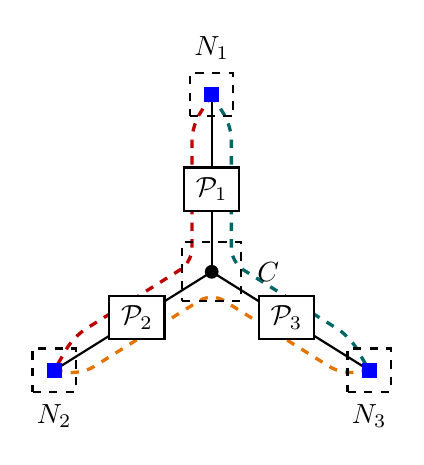
\begin{tikzpicture}[
            line/.style={thick},
            proc/.style={
                    rectangle, draw, fill=white, thick,
                    minimum width=0.7cm,
                    minimum height=0.55cm,
                    inner sep=1pt
                },
            endpoint/.style={
                    rectangle, fill=blue, draw=blue,
                    minimum size=0.18cm, inner sep=0pt
                },
            station/.style={
                    rectangle, draw, dashed, thick,
                    minimum width=0.55cm,
                    minimum height=0.55cm
                },
            center/.style={
                    circle, fill=black, draw=black,
                    minimum size=0.16cm, inner sep=0pt
                },
            pathline/.style={
                    very thick, dashed, rounded corners=5pt
                }
        ]
        \coordinate (C)  at (0,0);
        \coordinate (A1) at (0,2.25);
        \coordinate (A2) at (-2.0,-1.25);
        \coordinate (A3) at (2.0,-1.25);

        % Physical links
        \draw[line] (A1) -- (C);
        \draw[line] (A2) -- (C);
        \draw[line] (A3) -- (C);

        % Three end-to-end paths, offset for visual clarity
        \draw[pathline,red!75!black]
        (A1) -- (-0.25,1.85) -- (-0.25,0.12)
        -- (-1.75,-0.82) -- (A2);

        \draw[pathline,teal!80!black]
        (A1) -- (0.25,1.85) -- (0.25,0.12)
        -- (1.75,-0.82) -- (A3);

        \draw[pathline,orange!90!black]
        (A2) -- (-1.65,-1.30) -- (0,-0.27)
        -- (1.65,-1.30) -- (A3);

        % Pauli channels
        \node[proc] (P1) at (0,1.05) {$\mathcal P_1$};
        \node[proc] (P2) at (-0.95,-0.58) {$\mathcal P_2$};
        \node[proc] (P3) at (0.95,-0.58) {$\mathcal P_3$};

        % Central node
        \node[station,minimum width=0.75cm,
            minimum height=0.75cm] at (C) {};
        \node[center] at (C) {};
        \node[right=13pt] at (C) {$C$};

        % Peripheral monitors
        \node[station] at (A1) {};
        \node[endpoint] at (A1) {};
        \node[above=9pt] at (A1) {$N_1$};

        \node[station] at (A2) {};
        \node[endpoint] at (A2) {};
        \node[below=9pt] at (A2) {$N_2$};

        \node[station] at (A3) {};
        \node[endpoint] at (A3) {};
        \node[below=9pt] at (A3) {$N_3$};



    \end{tikzpicture}
    \caption{ Three-link star network with peripheral monitors \(N_1,N_2,N_3\) (blue squares) and a central node \(C\) (black circle). Each link \(\ell\) is modeled by an unknown Pauli channel \(\mathcal P_\ell \). The monitors provide SPAM capabilities, while \(C\) performs prescribed operations without supplying measurement outcomes to the tomography procedure. The red, teal, and orange dashed lines represent the three end-to-end paths
0        $N_1\!-\!C\!-\!N_2$, $N_1\!-\!C\!-\!N_3$, and $N_2\!-\!C\!-\!N_3$, respectively. }
    \label{fig:three-link-star}
\end{figure}


\textbf{End-to-End Distillation.}
Under the access constraints described above, we consider only
end-to-end (path-level) entanglement distillation between monitors. The local measurements required at both endpoints
by distillation protocols  can then be performed at the
monitors, with their outcomes accessible to the tomography procedure.
Link-level distillation would instead involve measurements at \(C\),
whose outcomes are unavailable to users. Even if the service provider
performs such distillation internally, we exclude it from our model
and use only measurement data obtained from path-level distillation. Specifically, we apply the double-selection protocol described in
\S~\ref{doub} to entangled pairs shared between monitors.
Besides conditionally retaining an output pair, the protocol
provides measurement statistics for estimating the input Bell-diagonal state.

We use these statistics in two estimation schemes.
Under the fidelity condition $F(\rho)>1/2$,
Lemma~\ref{lem:double-selection-statistics} allows all three
nontrivial parameters to be estimated using
\eqref{eq:double-selection-inversion}.
Alternatively, Observation~\ref{lem3} allows the $Z$-basis parameters
to be estimated from $p_Z$ alone without relying on this fidelity condition.
Suitable Clifford dressings extend the latter approach to
the $X$ and $Y$ components.
In both schemes, the estimated end-to-end correlations are
then combined to infer the individual link-level channel parameters.

The following assumption ensures the applicability of
Lemma~\ref{lem:double-selection-statistics} to  JCE.
Note that it is not required by MCE, which is based on
Observation~\ref{lem3}.

\begin{assumption}[Fidelity condition for JCE]
    \label{ass:fidelity-condition}
    The Bell-diagonal states
    $\rho_{12}$, $\rho_{13}$, $\rho_{\text{m},23}$, and
    $\rho_{\text{d},23}$, defined in
    \eqref{eq:direct-two-link-states},
    \eqref{eq:mergecast-undressed-state}, and
    \eqref{eq:mergecast-dressed-state}, each have fidelity greater
    than $1/2$ with respect to $\ket{\Phi^+}$.
\end{assumption}


\textbf{Objective.}
Given the three-link star network
\(\mathcal G\), our objective is to design end-to-end protocols that use distillation
measurement outcomes to estimate all link-level channel parameters
\(q_{P,\ell}\), for \(\ell\in\{1,2,3\}\) and
\(P\in\{X,Y,Z\}\). We quantify the estimation accuracy using the mean square error (MSE),
\begin{equation}
    \epsilon_{\mathrm{est}}
    \coloneqq
        \frac{1}{9}
        \sum_{\ell=1}^{3}
        \sum_{P\in\{X,Y,Z\}}
        \left(
        \widehat{q}_{P,\ell}-q_{P,\ell}
        \right)^2
    ,
\end{equation}
where \(\widehat{q}_{P,\ell}\) denotes the estimate of \(q_{P,\ell}\).
Our objective is to minimize this estimation error for a given measurement budget.
\begin{remark}[Extension to general network topologies]
    \label{rem:general-topology}
    Due to space limitations, this work focuses on the three-link star
    topology, which provides a fundamental setting in which individual
    link parameters can be estimated from end-to-end observations
    without access to the central node's measurement outcomes.

    The proposed framework can be naturally extended to more general
    quantum-network topologies without degree-two nodes based on two
    observations. First, any quantum network without degree-two nodes can
    be viewed as being composed of three-link star substructures. Second,
    for tomography purposes, two consecutive Pauli channels can be
    regarded as a single effective Pauli channel. We illustrate this
    extension through a larger-network example in \S~\ref{sub2}.
    A more comprehensive treatment is omitted due to space limitations.
\end{remark}


\section{Distillation-Assisted Network Tomography}
\label{sec:dist-qnt}

In this section, we develop a distillation-assisted tomography
protocol for the three-link star network.
\S\ref{subsec:direct-nt} first introduces direct pairwise
distillation and explains its identifiability limitation.
\S\ref{subsec:mergecast-nt} then presents a modified Mergecast
construction that provides estimation involving all three links.
\S\ref{subsec:Clifford-dressing} uses Clifford dressing to
obtain the additional estimation needed for complete estimation.
Finally, \S~\ref{linkpa} combines these measurement statistics
to construct JCE and MCE and establish the identifiability
of the three Pauli channels.
JCE requires the specified source-state fidelity condition
$F>1/2$, whereas MCE removes this requirement.

\subsection{Distillation-Assisted Unicast }
\label{subsec:direct-nt}



We begin with direct Unicast~\cite{Pirandola_2019} transmission between peripheral monitors,
where Unicast refers to single-path probe between one sender monitor and one receiver monitor (in the peripheral).
% where one monitor acts as the sender and the other as the
% receiver.
The three-link star network contains three two-link paths, each for
one pair of monitors as in Fig.~\ref{fig:three-link-star}. Consider the path
\(N_1\!-C\!-N_2\) shown in Fig.~\ref{fig:two-link-path}.
The Unicast procedure is as follows:
monitor \(N_1\) prepares a Bell pair \(\ket{\Phi^+}\), retains one qubit locally,
and sends the other to \(N_2\) through the Pauli channel \(\mathcal P_1\),
the central node \(C\), and the Pauli channel \(\mathcal P_2\).
The resulting state shared by monitor \(N_1\) and \(N_2\) is Bell diagonal,
as shown in Fig.~\ref{fig:two-link-path}.

\begin{figure}[tb]
    \centering
    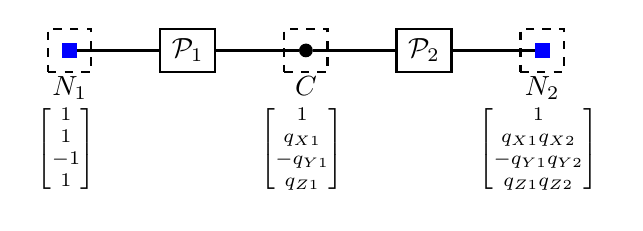
\begin{tikzpicture}[
            line/.style={thick},
            proc/.style={
                    rectangle,
                    draw,
                    thick,
                    minimum width=0.7cm,
                    minimum height=0.55cm,
                    inner sep=1pt
                },
            endpoint/.style={
                    rectangle,
                    fill=blue,
                    draw=blue,
                    minimum size=0.18cm,
                    inner sep=0pt
                },
            station/.style={
                    rectangle,
                    draw,
                    dashed,
                    thick,
                    minimum width=0.55cm,
                    minimum height=0.55cm
                },
            center/.style={
                    circle,
                    fill=black,
                    draw=black,
                    minimum size=0.16cm,
                    inner sep=0pt
                },
            state/.style={
                    font=\scriptsize,
                    align=center
                }
        ]

        % Coordinates
        \coordinate (C)  at (0,0);
        \coordinate (A1) at (-3,0);
        \coordinate (A2) at (3,0);

        % Central node
        \node[center] (center) at (C) {};
        \node[station] at (C) {};
        \node[below=6pt] at (C) {$C$};

        % Peripheral node A1
        \node[endpoint] (node1) at (A1) {};
        \node[station] at (A1) {};
        \node[below=6pt] at (A1) {$N_1$};

        % Peripheral node A2
        \node[endpoint] (node2) at (A2) {};
        \node[station] at (A2) {};
        \node[below=6pt] at (A2) {$N_2$};

        % Pauli channels
        \node[proc] (P1) at (-1.5,0) {$\mathcal P_1$};
        \node[proc] (P2) at ( 1.5,0) {$\mathcal P_2$};

        % Transmission path
        \draw[line] (node1) -- (P1) -- (center);
        \draw[line] (center) -- (P2) -- (node2);

        % Initial Bell-state vector at A1
        \node[state] at (-3,-1.25) {
            $\displaystyle
                \begin{bmatrix}
                    1  \\
                    1  \\
                    -1 \\
                    1
                \end{bmatrix}$
        };

        % State after channel P1, arriving at C
        \node[state] at (0,-1.25) {
            $
                \begin{bmatrix}
                    1       \\
                    q_{X1}  \\
                    -q_{Y1} \\
                    q_{Z1}
                \end{bmatrix}$
        };

        % State after channels P1 and P2, arriving at A2
        \node[state] at (3,-1.25) {
            $
                \begin{bmatrix}
                    1             \\
                    q_{X1}q_{X2}  \\
                    -q_{Y1}q_{Y2} \\
                    q_{Z1}q_{Z2}
                \end{bmatrix}$
        };

    \end{tikzpicture}

    \caption{
        Two-link path \(N_1\!-\!C\!-\!N_2\) through the central node \(C\).
        The column vectors below the nodes are the restricted
        Pauli--Liouville representation of the shared state at the
        corresponding transmission stage.
        By symmetry, the same protocol can be applied to the other
        two two-link paths, \(N_1- C- N_3\) and
        \(N_2- C- N_3\).
    }
    \label{fig:two-link-path}
\end{figure}
Applying the same procedure along the all three paths, including the other two \(N_2 \!-\!C\!-\!N_3\) and \(N_1\!-\!C\!-\!N_3\), gives the quantum states with restricted Pauli--Liouville representations as follows,
\begin{equation}
    \begin{aligned}
        \plket{\rho_{12}}
         & =
        \begin{bmatrix}
            1               &
            q_{X,1}q_{X,2}  &
            -q_{Y,1}q_{Y,2} &
            q_{Z,1}q_{Z,2}
        \end{bmatrix}^{T}, \\
        \plket{\rho_{13}}
         & =
        \begin{bmatrix}
            1               &
            q_{X,1}q_{X,3}  &
            -q_{Y,1}q_{Y,3} &
            q_{Z,1}q_{Z,3}
        \end{bmatrix}^{T}, \\
        \plket{\rho_{23}}
         & =
        \begin{bmatrix}
            1               &
            q_{X,2}q_{X,3}  &
            -q_{Y,2}q_{Y,3} &
            q_{Z,2}q_{Z,3}
        \end{bmatrix}^{T}.
    \end{aligned}
    \label{eq:direct-two-link-states}
\end{equation}

For each path, the two monitors independently generate three copies
of the shared state via the Unicast transmission above and then perform the double-selection protocol in~\S\ref{subsec:doub}.

Whenever the source state for distillation in~\eqref{eq:direct-two-link-states} satisfies the fidelity condition of
Lemma~\ref{lem:double-selection-statistics},
the double-selection
statistics in~\eqref{eq:double-selection-probabilities} \emph{uniquely estimate} its nontrivial Pauli correlations (e.g., the last three entries of \(\plket{\rho_{12}}\):
\(\widehat{q_{X,1}q_{X,2}}\),
\(\widehat{q_{Y,1}q_{Y,2}}\)
and \(\widehat{q_{Z,1}q_{Z,2}}\)). Thus, applying this
procedure to all three paths estimate any \(\widehat{q_{P, \ell}q_{P,\ell'}}\)
for any \(P\in\{X,Y,Z\}\)
and \((\ell, \ell') \in \{(1,2), (1,3), (2,3)\}\).


% \begin{equation}
%     q_{P,1}q_{P,2},
%     \quad
%     q_{P,1}q_{P,3},
%     \quad
%     q_{P,2}q_{P,3},
%     \quad P\in\{X,Y,Z\}.
% \end{equation}

% Insert Fig.~\ref{fig:two-link-path} here.

\paragraph{Identifiability challenge}

For each $P\in\{X,Y,Z\}$, the double-selection statistics yield
estimates of the pairwise products
$q_{P,1}q_{P,2}$, $q_{P,1}q_{P,3}$, and $q_{P,2}q_{P,3}$,
each involving an even number of factors.
From these three estimates, one can, for instance, estimate
the parameter $q_{P,1}$ as
$\pm\sqrt{
        \frac{
            \widehat{q_{P,1}q_{P,2}} \times \widehat{q_{P,1}q_{P,3}}
        }{
            \widehat{q_{P,2}q_{P,3}}
        }
    }$, with a sign ambiguity.
That is, there are two possible sign choices for each Pauli component,
across all three components giving up to eight choices in total.
This ambiguity suggests that this protocol alone cannot uniquely
identify all channels.


To resolve this sign ambiguity, we introduce a
Mergecast protocol in the following subsection,
which  generates estimates involving
all three links (i.e., products of an odd number of factors).
By combining the estimates with the ones in Unicast, we resolve
this sign ambiguity and uniquely estimate the channel parameters.

% In this scheme, only $\rho_{12}$ and $\rho_{13}$ are generated
% by direct transmission.
% For the remaining path $N_2\!-\!C\!-\!N_3$, we instead use
% undressed and Clifford-dressed Mergecast configurations,

% Instead, our protocol
% directly generates only \(\rho_{12}\) and \(\rho_{13}\).
% For the remaining path \(N_2\!-\!C\!-\!N_3\), we replace direct
% transmission with undressed and Clifford-dressed modified Mergecast
% configurations. 






\subsection{Distillation-Assisted Mergecast}
\label{subsec:mergecast-nt}
Fig.~\ref{fig:modified-mergecast} illustrates the Mergecast
protocol~\cite{wang2025quantumnetworktomographygeneral},
which introduces correlations involving all three links
to resolve the sign ambiguity.
We apply this protocol to the path $N_2\!-\!C\!-\!N_3$
and then use the double-selection protocol to estimate
the resulting Bell-diagonal state.
\begin{figure*}[tb]
    \centering
    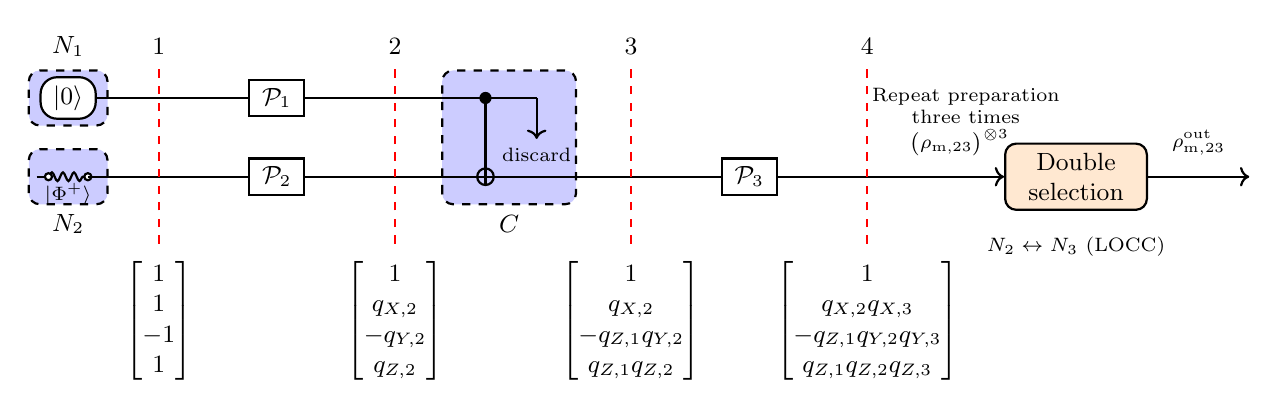
\begin{tikzpicture}[
            x=1cm,
            y=1cm,
            font=\small,
            wire/.style={thick},
            region/.style={
                    draw,
                    dashed,
                    thick,
                    rounded corners=4pt,
                    fill=blue!20
                },
            gate/.style={
                    draw,
                    thick,
                    fill=white,
                    minimum width=0.7cm,
                    minimum height=0.45cm,
                    inner sep=3pt
                },
            distillation/.style={
                    draw,
                    thick,
                    rounded corners=4pt,
                    fill=orange!18,
                    minimum width=1.8cm,
                    minimum height=0.8cm,
                    align=center
                },
            boundary/.style={draw=red,dashed,thick},
            state/.style={
                    anchor=north,
                    font=\small,
                    inner sep=0pt
                },
            ent/.style={
                    thick,
                    decorate,
                    decoration={
                            snake,
                            amplitude=0.55mm,
                            segment length=1.4mm
                        }
                }
        ]

        % Preparation regions and central node.
        \draw[region] (-0.15,0.65) rectangle (0.85,1.35);
        \draw[region] (-0.15,-0.35) rectangle (0.85,0.35);
        \draw[region] (5.10,-0.35) rectangle (6.80,1.35);

        % Auxiliary qubit from N_1 through P_1.
        \draw[wire] (0.35,1.00) -- (6.30,1.00);
        \node[gate,rounded corners=6pt]
        at (0.35,1.00) {$\ket{0}$};
        \node[gate] at (3.00,1.00) {$\mathcal P_1$};

        % Bell pair prepared at N_2.
        \draw[wire] (-0.05,0.00) -- (0.10,0.00);
        \draw[ent] (0.10,0.00) -- (0.60,0.00);
        \filldraw[draw=black,fill=white,thick]
        (0.10,0.00) circle (0.045);
        \filldraw[draw=black,fill=white,thick]
        (0.60,0.00) circle (0.045);
        \node[font=\scriptsize] at (0.35,-0.22)
        {$\ket{\Phi^+}$};

        % Traveling Bell qubit.
        \draw[wire] (0.60,0.00) -- (11.10,0.00);
        \node[gate] at (3.00,0.00) {$\mathcal P_2$};
        \node[gate] at (9.00,0.00) {$\mathcal P_3$};

        % CNOT at C: auxiliary control, traveling Bell qubit target.
        \fill (5.65,1.00) circle (2.2pt);
        \draw[thick] (5.65,1.00) -- (5.65,0.00);
        \draw[thick] (5.65,0.00) circle (0.105);
        \draw[thick] (5.65,-0.105) -- (5.65,0.105);
        \draw[thick] (5.545,0.00) -- (5.755,0.00);

        % Discard the auxiliary qubit.
        \draw[thick,->] (6.30,1.00) -- (6.30,0.48);
        \node[font=\scriptsize] at (6.30,0.28) {discard};

        % Node labels.
        \node at (0.35,1.65) {$N_1$};
        \node at (0.35,-0.60) {$N_2$};
        \node at (5.95,-0.60) {$C$};

        % Transmission slices.
        \foreach \x/\stage in {1.5/1,4.5/2,7.5/3,10.5/4}{
                \draw[boundary] (\x,-0.85) -- (\x,1.45);
                \node at (\x,1.65) {$\stage$};
            }

        % Bell-pair vectors in the ordered basis (II,XX,YY,ZZ).
        \node[state] at (1.5,-1.05) {
            $\begin{bmatrix}
                    1  \\
                    1  \\
                    -1 \\
                    1
                \end{bmatrix}$
        };

        \node[state] at (4.5,-1.05) {
            $\begin{bmatrix}
                    1        \\
                    q_{X,2}  \\
                    -q_{Y,2} \\
                    q_{Z,2}
                \end{bmatrix}$
        };

        \node[state] at (7.5,-1.05) {
            $\begin{bmatrix}
                    1               \\
                    q_{X,2}         \\
                    -q_{Z,1}q_{Y,2} \\
                    q_{Z,1}q_{Z,2}
                \end{bmatrix}$
        };

        \node[state] at (10.5,-1.05) {
            $\begin{bmatrix}
                    1                      \\
                    q_{X,2}q_{X,3}         \\
                    -q_{Z,1}q_{Y,2}q_{Y,3} \\
                    q_{Z,1}q_{Z,2}q_{Z,3}
                \end{bmatrix}$
        };

        % Three independent preparations supply the distillation input.
        \node[font=\scriptsize,align=center] at (11.75,0.90)
        {Repeat preparation\\three times};

        \node[distillation] (DS) at (13.15,0.00)
        {Double\\selection};

        \draw[wire,->] (11.10,0.00) -- (DS.west)
        node[midway,above=4pt,font=\scriptsize]
        {$\bigl(\rho_{\text{m,}23}\bigr)^{\otimes3}$};

        \node[font=\scriptsize,below=6pt] at (DS.south)
        {$N_2\leftrightarrow N_3$ (LOCC)};

        % Conditionally retained output pair.
        \draw[wire,->] (DS.east) -- (15.35,0.00)
        node[midway,above=4pt,font=\scriptsize]
        {$\rho_{\text{m},23}^{\mathrm{out}}$};

    \end{tikzpicture}

    \caption{
        Mergecast preparation followed by double-selection protocol.
        Slices 1--4 illustrate the entanglement-generation procedure, adapted
        from the Mergecast protocol in
        \cite{wang2025quantumnetworktomographygeneral}.
        The column vectors give the restricted Pauli--Liouville
        representations of the reduced two-qubit state.
        The preparation is repeated independently three times, after which
        monitors \(N_2\) and \(N_3\) perform double-selection protocol to
        distill a retained entangled pair and estimate the input-state
        parameters from the measurement statistics.
    }
    \label{fig:modified-mergecast}
\end{figure*}
The procedure is as follows.
\begin{enumerate}
    \item Node \(N_2\) prepares \(\ket{\Phi^+}\), retains one qubit,
          and sends the other to \(C\) through \(\mathcal P_2\). Meanwhile,
          \(N_1\) sends an auxiliary qubit in \(\ket{0}\) to \(C\) through
          \(\mathcal P_1\).

    \item Node \(C\) applies a CNOT with the auxiliary qubit as the
          control and the Bell-pair qubit as the target. It then traces out (i.e., discard)
          the control and forwards the target to \(N_3\) through
          \(\mathcal P_3\).
    \item After generating three independent copies from repeating steps 1) and 2), node \(N_2\) and
          \(N_3\) perform double-selection protocol.
\end{enumerate}

Before distillation, each source state shared by \(N_2\) and \(N_3\) is
\begin{equation}
    \plket{\rho_{\text{m},23}}
    =
    \begin{bmatrix}
        1                      &
        q_{X,2}q_{X,3}         &
        -q_{Z,1}q_{Y,2}q_{Y,3} &
        q_{Z,1}q_{Z,2}q_{Z,3}
    \end{bmatrix}^{ T}.
    \label{eq:mergecast-undressed-state}
\end{equation}


By Lemma~\ref{lem:double-selection-statistics}, the double-selection
statistics yield estimates of the nontrivial Pauli coefficients
of $\rho_{\text{m},23}$.
For example, combining the resulting estimate of
$q_{Z,1}q_{Z,2}q_{Z,3}$ with the previously obtained estimate
of $q_{Z,1}q_{Z,2}$ gives
\(
\widehat{q}_{Z,3}
\coloneqq
\frac{
    \widehat{q_{Z,1}q_{Z,2}q_{Z,3}}
}{
    \widehat{q_{Z,1}q_{Z,2}}
},
\)
This illustrates how combining the estimates from the two protocols
resolves the sign ambiguity.
Further details are presented in \S~\ref{linkpa}.

% The double-selection statistics determine the three-link correlation
% \(q_{Z,1}q_{Z,2}q_{Z,3}\). Combining it with the pairwise correlations
% obtained from direct distillation gives
% \begin{equation}
% \begin{aligned}
%     q_{Z,1}
%     &=
%     \frac{
%         (q_{Z,1}q_{Z,2})(q_{Z,1}q_{Z,3})
%     }{
%         q_{Z,1}q_{Z,2}q_{Z,3}
%     },\\
%     q_{Z,2}
%     &=
%     \frac{
%         q_{Z,1}q_{Z,2}q_{Z,3}
%     }{
%         q_{Z,1}q_{Z,3}
%     },\\
%     q_{Z,3}
%     &=
%     \frac{
%         q_{Z,1}q_{Z,2}q_{Z,3}
%     }{
%         q_{Z,1}q_{Z,2}
%     }.
% \end{aligned}
% \end{equation}

To recover the remaining parameters
\(q_{X,\ell}\) and \(q_{Y,\ell}\), we need to access correlations
in other Pauli bases. We achieve this through channel dressing,
as described below.


\begin{remark}[Fidelity inefficiency of the Mergecast protocol]
    Although this Mergecast operation may
    reduce the fidelity of the final source state in~\eqref{eq:mergecast-undressed-state} shared by node \(N_2\) and \(N_3\), it
    provides information that cannot be obtained from Unicast and resolve the sign ambiguity issue.
    In other words, it trades some end-to-end
    fidelity for the identifiability.
\end{remark}

\subsection{Clifford-Dressed Pauli Channels}
\label{subsec:Clifford-dressing}

We adapt the channel-dressing technique of Wang et al.~\cite{wang2025quantumnetworktomographygeneral} to the
Mergecast protocol.
Specifically, in Fig.~\ref{fig:modified-mergecast},
we apply different Clifford
dressings to \(\mathcal P_2\) and \(\mathcal P_3\), while leaving
\(\mathcal P_1\) unchanged.
Dressing the channels is equivalent to change
    input and output bases of the channels, providing the statistics for estimating other channel parameters.



The dressing uses the Hadamard gate \(H\) and phase gate \(S\).
Both are Clifford gates, which bijectively map Pauli operators to Pauli
operators up to a sign under
conjugation~\cite{Gottesman1998Heisenberg}.
Ignoring signs, \(H\) exchanges \(X\) and \(Z\), while \(S\)
exchanges \(X\) and \(Y\). Together, these exchanges generate all
permutations of \(\{X,Y,Z\}\).
When a Pauli channel is dressed by a Clifford gate and its Hermitian conjugate,
the signs cancel, so the dressing simply permutes its PTM
eigenvalues. We use the Clifford gates \(SHS\) and \(S\) to define
\begin{equation}
\begin{aligned}
\mathcal P_2^{(SHS)}
\coloneqq SHS\circ\mathcal P_2\circ(SHS)^\dagger,\
\mathcal P_3^{(S)}
&\coloneqq S\circ\mathcal P_3\circ S^\dagger.
\end{aligned}
\label{eq:dressed-pauli-channels}
\end{equation}
These dressings exchange the \(Y\) and \(Z\) eigenvalues of
\(\mathcal P_2\), and the \(X\) and \(Y\) eigenvalues of
\(\mathcal P_3\), respectively, as illustrated in
Fig.~\ref{fig:pauli-channel-dressing}.

\begin{figure}[tb]
    \centering
    \resizebox{\columnwidth}{!}{%
        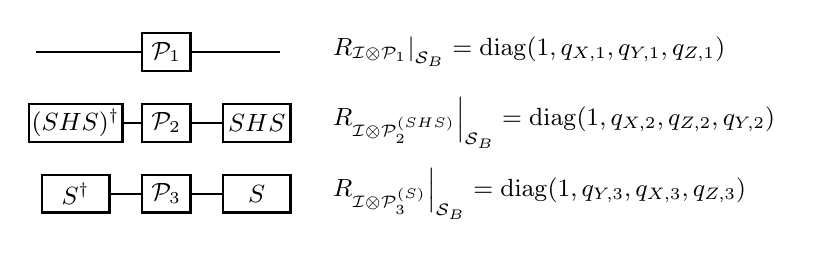
\begin{tikzpicture}[
                x=1cm,
                y=1cm,
                font=\small,
                wire/.style={draw=black,thick},
                gate/.style={
                        draw=black,
                        thick,
                        fill=white,
                        minimum width=0.62cm,
                        minimum height=0.48cm,
                        inner sep=1pt
                    },
                widegate/.style={gate,minimum width=0.86cm}
            ]

            % Link 1 remains undressed.
            \draw[wire,-] (0.15,1.25) -- (3.25,1.25);
            \node[gate] at (1.80,1.25) {$\mathcal P_1$};
            \node[anchor=west] at (3.75,1.25) {
                $\left.R_{\mathcal I\otimes\mathcal P_1}\right|_{\mathcal S_B}
                    =\operatorname{diag}(1,q_{X,1},q_{Y,1},q_{Z,1})$
            };

            % Apply (SHS)^\dagger before P_2 and SHS after P_2.
            \draw[wire,-] (0.15,0.35) -- (3.25,0.35);
            \node[widegate] at (0.65,0.35) {$(SHS)^\dagger$};
            \node[gate] at (1.80,0.35) {$\mathcal P_2$};
            \node[widegate] at (2.95,0.35) {$SHS$};
            \node[anchor=west] at (3.75,0.35) {
                $\left.R_{\mathcal I\otimes\mathcal P_2^{(SHS)}}\right|_{\mathcal S_B}
                    =\operatorname{diag}(1,q_{X,2},q_{Z,2},q_{Y,2})$
            };

            % Apply S^\dagger before P_3 and S after P_3.
            \draw[wire,-] (0.35,-0.55) -- (3.25,-0.55);
            \node[widegate] at (0.65,-0.55) {$S^\dagger$};
            \node[gate] at (1.80,-0.55) {$\mathcal P_3$};
            \node[widegate] at (2.95,-0.55) {$S$};
            \node[anchor=west] at (3.75,-0.55) {
                $\left.R_{\mathcal I\otimes\mathcal P_3^{(S)}}\right|_{\mathcal S_B}
                    =\operatorname{diag}(1,q_{Y,3},q_{X,3},q_{Z,3})$
            };

        \end{tikzpicture}%
    }
    \caption{
        Link-dependent Clifford dressing used in the modified Mergecast
        protocol.
        Each channel $\mathcal P_\ell$ is preceded by $U_\ell^\dagger$
        and followed by $U_\ell$, with $U_1=I$, $U_2=SHS$, and $U_3=S$.
        Thus, $\mathcal P_1$ remains unchanged, while the PTM eigenvalues
        of $\mathcal P_2$ and $\mathcal P_3$ are permuted as
        $(q_{X,2},q_{Y,2},q_{Z,2})
            \mapsto(q_{X,2},q_{Z,2},q_{Y,2})$
        and
        $(q_{X,3},q_{Y,3},q_{Z,3})
            \mapsto(q_{Y,3},q_{X,3},q_{Z,3})$, respectively.
        These dressings allow the Mergecast protocol to access the
        mixed products $q_{Z,1}q_{Z,2}q_{X,3}$ and
        $q_{Z,1}q_{Y,2}q_{Z,3}$, which provide the additional information
        needed to resolve the remaining sign ambiguities.
    }
    \label{fig:pauli-channel-dressing}
\end{figure}

Replacing \(\mathcal P_2\) and \(\mathcal P_3\) with these dressed
channels in the Mergecast-based distillation protocol produces
\begin{equation}
    \plket{\rho_{\text{d},23}}
    =
    \begin{bmatrix}
        1                      &
        q_{X,2}q_{Y,3}         &
        -q_{Z,1}q_{Z,2}q_{X,3} &
        q_{Z,1}q_{Y,2}q_{Z,3}
    \end{bmatrix}^{\mathsf T}.
    \label{eq:mergecast-dressed-state}
\end{equation}
By Lemma~\ref{lem:double-selection-statistics}, the double-selection
statistics  recovers the
nontrivial Pauli coefficients of \(\rho_{\text{d},23}\).
In particular, the last two coefficients provide the information
needed to determine \(q_{X,3}\) and \(q_{Y,2}\).
Together with the direct and undressed Mergecast measurements,
they enable the complete channel estimation described next.

\subsection{Link-Parameter Estimation}
\label{linkpa}
\paragraph{Joint-Coincidence Estimator (JCE)}
Under Assumption~\ref{ass:fidelity-condition} on source-state fidelity, JCE combines the estimates obtained from the four configurations
to estimate the individual channel parameters.


By Lemma~\ref{lem:double-selection-statistics}, the double-selection
statistics of the directly generated states $\rho_{12}$ and
$\rho_{13}$ yield estimators $\widehat{\pi}_{12}^{(P)}$ and
$\widehat{\pi}_{13}^{(P)}$ of the pairwise products defined as follows,
\begin{equation}
    \begin{aligned}
        \pi_{12}^{(P)}
         & \coloneqq q_{P,1}q_{P,2},\,
        \pi_{13}^{(P)}
        \coloneqq q_{P,1}q_{P,3},
        \, P\in\{X,Y,Z\}.
    \end{aligned}
    \label{eq:direct-correlations}
\end{equation}
Similarly, the double-selection statistics of the undressed
Mergecast state $\rho_{\text{m},23}$ yield an estimator
$\widehat{\tau}_Z$ of the three-link correlation
\[
    \tau_Z\coloneqq q_{Z,1}q_{Z,2}q_{Z,3}.
\]
Combining these estimates, we define
\begin{equation}
    \begin{aligned}
        \widehat{q}_{Z,1}
        \coloneqq
        \frac{\widehat{\pi}_{12}^{(Z)}
            \widehat{\pi}_{13}^{(Z)}}{\widehat{\tau}_Z},
        \widehat{q}_{Z,2}
        \coloneqq
        \frac{\widehat{\tau}_Z}{\widehat{\pi}_{13}^{(Z)}},
        \widehat{q}_{Z,3}
        \coloneqq
        \frac{\widehat{\tau}_Z}{\widehat{\pi}_{12}^{(Z)}}.
    \end{aligned}
    \label{eq:z-parameter-reconstruction}
\end{equation}

To estimate the remaining parameters, we use the double-selection
statistics of the dressed Mergecast state $\rho_{\text{d},23}$.
These statistics yield estimators $\widehat{\mu}_X$ and
$\widehat{\mu}_Y$ of
\[
    \mu_X\coloneqq q_{Z,1}q_{Z,2}q_{X,3},
    \qquad
    \mu_Y\coloneqq q_{Z,1}q_{Y,2}q_{Z,3}.
\]
Dividing these estimates by the corresponding  estimates gives
\begin{equation}
    \widehat{q}_{X,3}
    \coloneqq
    \frac{\widehat{\mu}_X}{\widehat{\pi}_{12}^{(Z)}},
    \qquad
    \widehat{q}_{Y,2}
    \coloneqq
    \frac{\widehat{\mu}_Y}{\widehat{\pi}_{13}^{(Z)}}.
    \label{eq:reference-parameter-reconstruction}
\end{equation}
These expressions provide estimates of both the magnitude and sign
of one parameter in each of the $X$ and $Y$ sectors.
The remaining parameters are then estimated sequentially as
\begin{equation}
    \begin{aligned}
        \widehat{q}_{X,1}
         & \coloneqq
        \frac{\widehat{\pi}_{13}^{(X)}}{\widehat{q}_{X,3}},
         &
        \widehat{q}_{X,2}
         & \coloneqq
        \frac{\widehat{\pi}_{12}^{(X)}}{\widehat{q}_{X,1}}, \\
        \widehat{q}_{Y,1}
         & \coloneqq
        \frac{\widehat{\pi}_{12}^{(Y)}}{\widehat{q}_{Y,2}},
         &
        \widehat{q}_{Y,3}
         & \coloneqq
        \frac{\widehat{\pi}_{13}^{(Y)}}{\widehat{q}_{Y,1}}.
    \end{aligned}
    \label{eq:remaining-parameter-reconstruction}
\end{equation}

Finally, applying the transformation in
Lemma~\ref{lem:bell-pauli-transformation} gives estimators
of the Pauli-error probabilities of each channel:
\begin{equation}
    \begin{bmatrix}
        \widehat{A}_\ell \\
        \widehat{B}_\ell \\
        \widehat{C}_\ell \\
        \widehat{D}_\ell
    \end{bmatrix}
    \coloneqq
    W^{ T}
    \begin{bmatrix}
        1                     \\
        \widehat{q}_{X,\ell}  \\
        -\widehat{q}_{Y,\ell} \\
        \widehat{q}_{Z,\ell}
    \end{bmatrix},
    \qquad \ell\in\{1,2,3\}.
    \label{eq:channel-probability-reconstruction}
\end{equation}

To summarize, ~\eqref{eq:z-parameter-reconstruction}--%
\eqref{eq:remaining-parameter-reconstruction} give estimates
of the link parameters, while~\eqref{eq:channel-probability-reconstruction} gives the
corresponding estimates of the Pauli-error probabilities.
The corresponding exact estimation establishes the
following identifiability result.

\begin{theorem}[Estimation with a fidelity assumption]
\label{cor:three-link-identifiability}
Under Assumptions~\ref{ass:nonzero-eigenvalues}
and~\ref{ass:fidelity-condition}, all nine link-level PTM
eigenvalues, and hence all three Pauli channels, are uniquely
identifiable from double-selection statistics through
~\eqref{eq:z-parameter-reconstruction}--%
\eqref{eq:remaining-parameter-reconstruction}, by combining
the Unicast{} and Mergecast{} protocols with link-dependent
Clifford dressing.
\end{theorem}

The fidelity assumption can be relaxed when estimating
$q_{Z,1}$, $q_{Z,2}$, and $q_{Z,3}$, as follows.

\begin{observation}[Estimation of the link parameters $q_{Z,\ell}$]
\label{obs:z-link-reconstruction}
The exact
$Z$-basis coincidence probabilities obtained from
$\rho_{12}$, $\rho_{13}$, and $\rho_{\text{m,}23}$ uniquely
determine $q_{Z,1}$, $q_{Z,2}$, and $q_{Z,3}$ without
Assumption~\ref{ass:fidelity-condition}.
The corresponding estimators are given by~\eqref{eq:z-parameter-reconstruction}.
\end{observation}

Indeed, Observation~\ref{lem3} allows the products
$q_{Z,1}q_{Z,2}$, $q_{Z,1}q_{Z,3}$, and
$q_{Z,1}q_{Z,2}q_{Z,3}$ to be estimated from the
corresponding $Z$-basis measurement statistics alone.
These products suffice to estimate all three $q_{Z,\ell}$.

\paragraph{Marginal-Coincidence Estimator (MCE)}
Building on Observation~\ref{obs:z-link-reconstruction},
MCE removes the
fidelity requirement, constituting another key contribution of this work.
We retain~\eqref{eq:z-parameter-reconstruction} for
estimating $q_{Z,\ell}$ and extend the same estimation
to $q_{X,\ell}$ and $q_{Y,\ell}$ through uniform Clifford dressing.
This scheme uses only the $Z$-basis measurement statistics, leaving the other
information unused.

                                                                                                                                                                                                                                                                                                                                                                                                                                                                                                                                                                                                                                                                                                                                                                                                                                                                                                                                                                                                                                                                                                                                                                                                                                                                                                                                                                                                                                                                                                                                                                                                                                                                                                                                                                                                                                                                                                                                                                                                                                                                                                                                                                                                                                                                                                                                                                                                                                                                                                                                                                                                                                                                                                                                                                                                                                                                                                                                                                                                                                                                                                                                                                                                                                                                                                                                                                                                                                                                                                                                                                                                                                                                                                                                                                                                                                                                                                                                                                                                                                                                                                                                                                                                                                                                                                                                                                                                                                                                                                                                                                                                                                                                                                                                                                                                                                                                                                                                                                                                                                                                                                                                                                                                                                                                                                                                                                                                                                                                                                                                                                                                                                                                                                                                                                                                                                                                                                                                                                                                                                                                                                                            
                                                                                                                                                                                                                                                                                                                                                                                                                                                                                                                                                                                                                                                                                                                                                                                                                                                                                                                                                                                                                                                                                                                                                                                                                                                                                                                                                                                                                                                                                                                                                                                                                                                                                                                                                                                                                                                                                                                                                                                                                                                                                                                                                                                                                                                                                                                                                                                                                                                                                                                                                                                                                                                                                                                                                                                                                                                                                                                                                                                                                                                                                                                                                                                                                                                                                                                                                                                                                                                                                                                                                                                                                                                                                                                                                                                                                                                                                                                                                                                                                                                                                                                                                                                                                                                                                                                                                                                                                                                                                                                                                                                                                                                                                                                                                                                                                                                                                                                                                                                                                                                                                                                                                                                                                                                                                                                                                                                                                                                                                                                                                                                                                                                                                                                                                                                                                                                                                                                                                                                                                                                                                                                                 
\begin{figure}[tb]
    \centering
    \resizebox{\columnwidth}{!}{%
        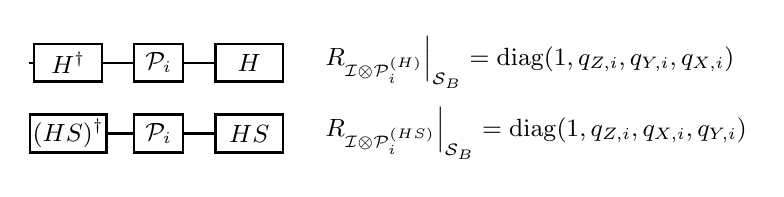
\begin{tikzpicture}[
                x=1cm,
                y=1cm,
                font=\small,
                wire/.style={draw=black,thick},
                gate/.style={
                        draw=black,
                        thick,
                        fill=white,
                        minimum width=0.62cm,
                        minimum height=0.48cm,
                        inner sep=1pt
                    },
                widegate/.style={gate,minimum width=0.86cm}
            ]

            % H dressing: the effective Z parameter is q_{X,i}.
            \draw[wire] (0.15,0.35) -- (3.25,0.35);
            \node[widegate] at (0.65,0.35) {$H^\dagger$};
            \node[gate] at (1.80,0.35) {$\mathcal P_i$};
            \node[widegate] at (2.95,0.35) {$H$};
            \node[anchor=west] at (3.75,0.35) {
                $\left.R_{\mathcal I\otimes\mathcal P_i^{(H)}}\right|_{\mathcal S_B}
                    =\operatorname{diag}(1,q_{Z,i},q_{Y,i},q_{X,i})$
            };

            % HS dressing: the effective Z parameter is q_{Y,i}.
            \draw[wire] (0.15,-0.55) -- (3.25,-0.55);
            \node[widegate] at (0.65,-0.55) {$(HS)^\dagger$};
            \node[gate] at (1.80,-0.55) {$\mathcal P_i$};
            \node[widegate] at (2.95,-0.55) {$HS$};
            \node[anchor=west] at (3.75,-0.55) {
                $\left.R_{\mathcal I\otimes\mathcal P_i^{(HS)}}\right|_{\mathcal S_B}
                    =\operatorname{diag}(1,q_{Z,i},q_{X,i},q_{Y,i})$
            };

        \end{tikzpicture}%
    }
    \caption{
        Clifford dressing of the Pauli channel $\mathcal P_i$ and the
        resulting permutations of its PTM eigenvalues.
        The upper and lower circuits implement the $H$ and $HS$
        dressings, respectively, with the corresponding restricted
        PTMs shown on the right.
        These dressings give $q_{Z,i}^{(H)}=q_{X,i}$ and
        $q_{Z,i}^{(HS)}=q_{Y,i}$, allowing the original $X$ and $Y$
        parameters to be estimated through the effective $Z$ parameter.
    }
    \label{fig:pauli-channel-dressing2}
\end{figure}

    To estimate $q_{X,\ell}$ and $q_{Y,\ell}$, we apply each of the
    Clifford dressings shown in Fig.~\ref{fig:pauli-channel-dressing2}
    uniformly to all three channels in the network.
    This differs from JCE, which applies different
    dressings to different channels in Mergecast.
    The $H$ and $HS$ dressings map $q_{X,\ell}$ and $q_{Y,\ell}$,
    respectively, to the effective $Z$ eigenvalues  of the dressed channels:
    \begin{equation}
        q_{Z,\ell}^{(H)}=q_{X,\ell},
        \qquad
        q_{Z,\ell}^{(HS)}=q_{Y,\ell},
        \qquad \forall \ell\in\{1,2,3\}.
    \end{equation}
For each dressing, we apply the same transformation to all
three links and repeat the Unicast{} and undressed Mergecast{}
procedures with the dressed channels.
Observation~\ref{lem3} then yields estimates
$\widehat{\pi}_{12}^{(P)}$, $\widehat{\pi}_{13}^{(P)}$, and
$\widehat{\tau}_P$ of $q_{P,1}q_{P,2}$, $q_{P,1}q_{P,3}$,
and $q_{P,1}q_{P,2}q_{P,3}$, respectively, for $P\in\{X,Y\}$.
Substituting these estimates into~\eqref{eq:z-parameter-reconstruction}, with $Z$ replaced
by $X$ or $Y$, gives
\begin{equation}
\begin{aligned}
    \widehat{q}_{X,1}
    &\coloneqq
    \frac{\widehat{\pi}_{12}^{(X)}
          \widehat{\pi}_{13}^{(X)}}{\widehat{\tau}_X},
    \quad
    \widehat{q}_{X,2}
    \coloneqq
    \frac{\widehat{\tau}_X}{\widehat{\pi}_{13}^{(X)}},
    \quad
    \widehat{q}_{X,3}
    \coloneqq
    \frac{\widehat{\tau}_X}{\widehat{\pi}_{12}^{(X)}},\\
    \widehat{q}_{Y,1}
    &\coloneqq
    \frac{\widehat{\pi}_{12}^{(Y)}
          \widehat{\pi}_{13}^{(Y)}}{\widehat{\tau}_Y},
    \quad
    \widehat{q}_{Y,2}
    \coloneqq
    \frac{\widehat{\tau}_Y}{\widehat{\pi}_{13}^{(Y)}},
    \quad
    \widehat{q}_{Y,3}
    \coloneqq
    \frac{\widehat{\tau}_Y}{\widehat{\pi}_{12}^{(Y)}}.
\end{aligned}
\label{eq22}
\end{equation}
Together with~\eqref{eq:z-parameter-reconstruction},
these estimators give the following estimation result.
\begin{theorem}[Estimation without a fidelity assumption]
        \label{thm:reconstruction-without-fidelity}
        Even without Assumption~\ref{ass:fidelity-condition}, all link-level
        PTM eigenvalues of these three Pauli channels in the star network remain uniquely
        identifiable from double-selection statistics  via~\eqref{eq:z-parameter-reconstruction} and~\eqref{eq22} by combining
        Clifford dressing with the Unicast and Mergecast protocols.
    \end{theorem}
\textcolor{blue}{
The two estimators establish identifiability under different conditions and exhibit a trade-off between measurement efficiency and applicability. JCE exploits joint $X/Z$ coincidence statistics and link-dependent Clifford dressing to estimate all nine channel parameters using four measurement configurations, but requires the source-state fidelity condition $F>1/2$. In contrast, MCE relies only on $Z$-basis coincidence statistics and uniform Clifford dressing, removing the fidelity requirement at the cost of increasing the number of configurations from four to nine. Consequently, each complete round requires 16 measured qubits for JCE and 36 for MCE. Thus, JCE is more resource-efficient in terms of configurations and measurements per round when the fidelity condition holds, whereas MCE offers broader applicability without this condition. The statistical efficiency of the two estimators under equal measurement budgets is further evaluated in \S~\ref{sec:problem-formulation}.}
% Copy this section into the manuscript, or use \input{...}.
% Required in the manuscript preamble:
% \usepackage{amsmath,amssymb,graphicx,booktabs,tikz,placeins}
% \usetikzlibrary{arrows.meta}
% Put the accompanying figures directory beside the main manuscript.

\section{Numerical Experiments}
\label{sec:numerical-experiments}

We evaluate the proposed joint-coincidence estimator (\jce) and marginal-coincidence estimator (\mce) through quantum circuit simulations using Qiskit~\cite{javadiabhari2024quantumcomputingqiskit}. We first consider a three-link star network and compare the estimation accuracy of the proposed methods with two existing tomography methods: \mergecast~\xw{cite}, which supports general Pauli-channel tomography, and Multicast~\cite{deandrade2024quantumnetworktomography}, which is restricted to depolarizing-channel tomography. The comparisons are conducted under different measurement budgets and assumptions about prior channel knowledge. We also examine the number of fidelity-improved entangled pairs retained during distillation to demonstrate the dual functionality of the proposed methods. We then extend \jce to a six-link triangular network \xw{(Figure~\ref{})} to evaluate its applicability beyond the three-link star topology. Estimation accuracy is quantified by the mean squared error (MSE) of the estimated Pauli-channel parameters, with measurement outcomes generated during distillation reused for channel estimation.
\subsection{Performance in a Three-Link Star Network}
\label{subsec:star-experiments}

\subsubsection{Network setting}
We consider a three-link star network in which each link is modeled by a depolarizing channel with \(q_{X,\ell}=q_{Y,\ell}=q_{Z,\ell}\). The channel parameters are \(q_{P,1}=0.88\), \(q_{P,2}=0.86\), and \(q_{P,3}=0.84\) for links 1, 2, and 3, respectively. 

Local gates and measurements are assumed to be ideal.
We consider two estimation settings that differ in whether the
depolarizing structure is known beforehand. Each measurement
budget is evaluated using 1000 Qiskit trials.

The measurement budget counts all measured qubits, including
those measured in rejected distillation attempts, and excludes
retained output pairs and unmeasured qubits discarded at
the central node.
For JCE and MCE, these measurements are part of distillation;
for the baseline protocols, they are dedicated to tomography.
Thus, ``free distillation measurement'' denotes reuse without
additional tomography measurements, rather than zero
physical resource consumption.

\paragraph{Without a depolarizing prior.}
Although the simulated channels are depolarizing, the estimators  in Fig.~\ref{fig:star-tomography-comparisons}(a)
are only supplied with the general Pauli-channel model.
JCE, MCE, and Mergecast therefore independently
estimate all nine parameters
$\{q_{P,\ell}:P\in\{X,Y,Z\},\,\ell=1,2,3\}$,
without imposing equality between the three Pauli components.

A complete round uses four, nine, and nine configurations for
JCE, MCE, and Mergecast, respectively, and 
16, 36, and 9 measurements.
Their performance is compared at equal measurement budgets.



The MSE decreases as the measurement budget increases.
Mergecast achieves the lowest MSE in this setting, while
JCE is more accurate than MCE at the same measurement budget.
The proposed estimators additionally use their measurement
records for distillation, producing the retained entangled
pairs discussed below.
% Required packages: \usepackage{booktabs,threeparttable}
% Table fragment; requires \usepackage{booktabs}.
\begin{table}
\centering
\caption{Mean numbers of fidelity-improved Bell pairs over 1,000 Qiskit trials at  approximately $200,000$ measurements per method. JCE and MCE use independent records, with four and nine configurations per round, respectively. Fidelities describe theoretical input and accepted-output ensembles. Mergecast retains no distilled outputs.}
\label{tab:three-methods-mean-retained-pairs}
\small
\setlength{\tabcolsep}{4pt}
\begin{tabular}{ccccc}
\toprule
$F_{\mathrm{in}}$ & $F_{\mathrm{out}}$ & JCE & MCE & Mergecast \\
\midrule
0.817600 & 0.901788 & 7,618 & 10,161 & 0 \\
0.804400 & 0.891105 & 7,355 & 9,800 & 0 \\
0.748456 & 0.843859 & 12,713 & 8,477 & 0 \\
\midrule
\multicolumn{2}{c}{Total} & \textbf{27,687} & \textbf{28,438} & \textbf{0} \\
\bottomrule
\end{tabular}
\end{table}

\begin{figure*}[tb]
\centering

\begin{subfigure}[t]{0.24\textwidth}
    \centering
    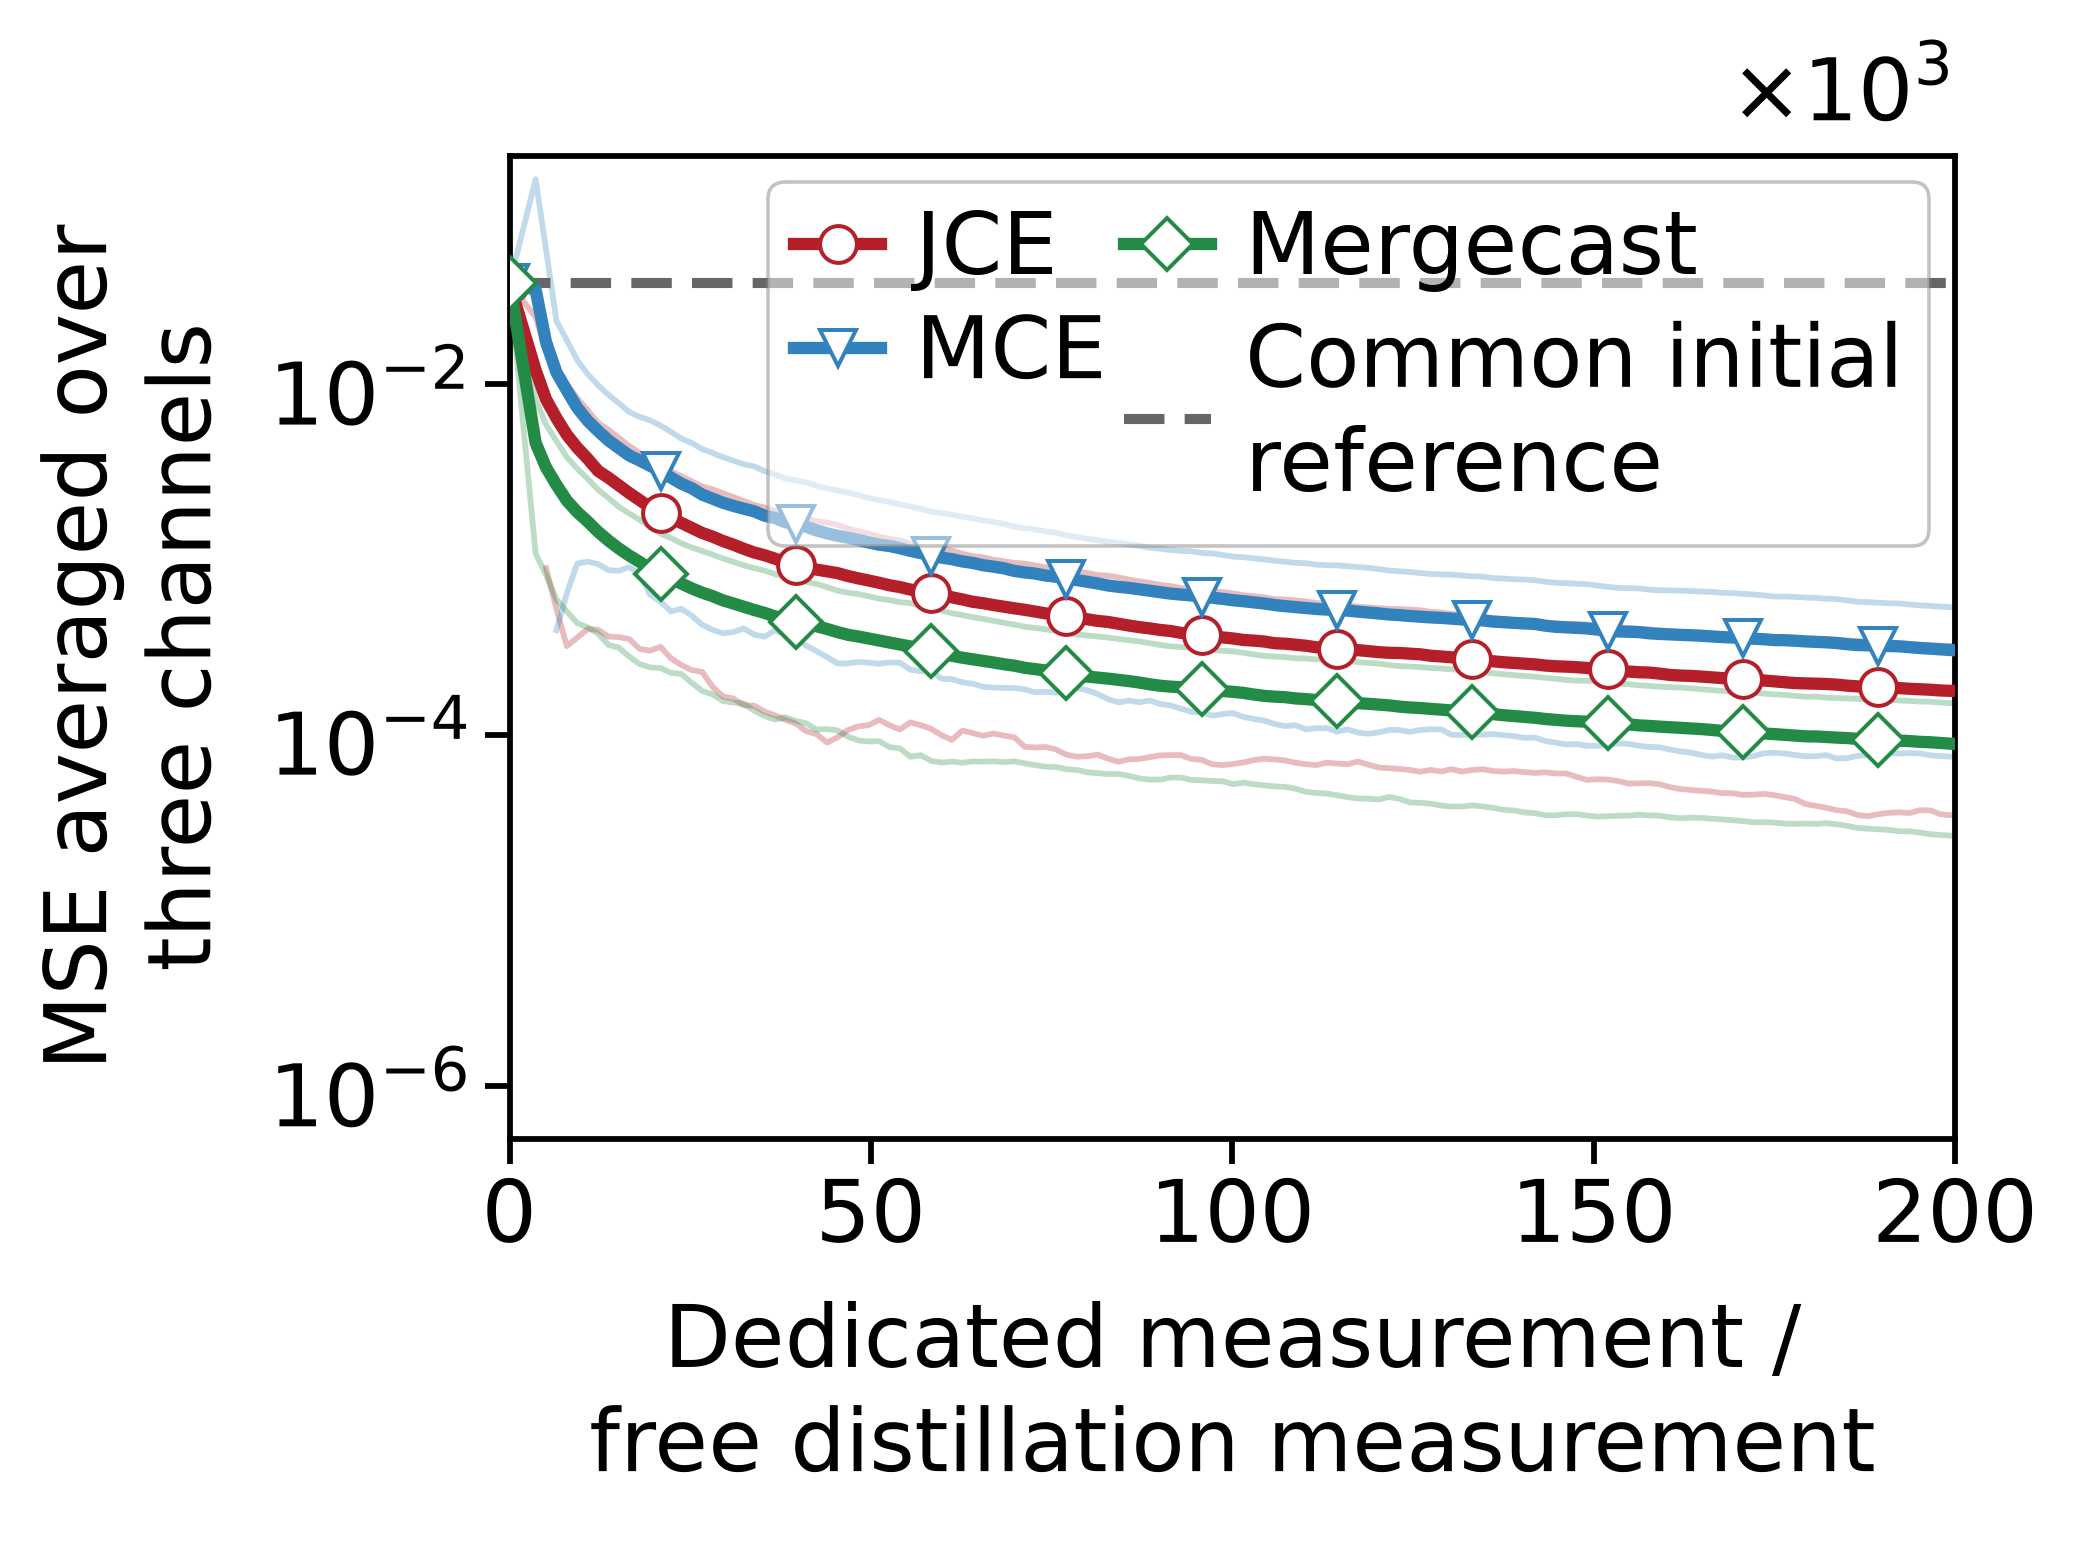
\includegraphics[width=\linewidth]
    {figures/star_three_methods_equal_measured_qubits.png}
    \caption{Without a depolarizing prior.}
    \label{fig:star-without-depolarizing-prior}
\end{subfigure}
\hfill
\begin{subfigure}[t]{0.24\textwidth}
    \centering
    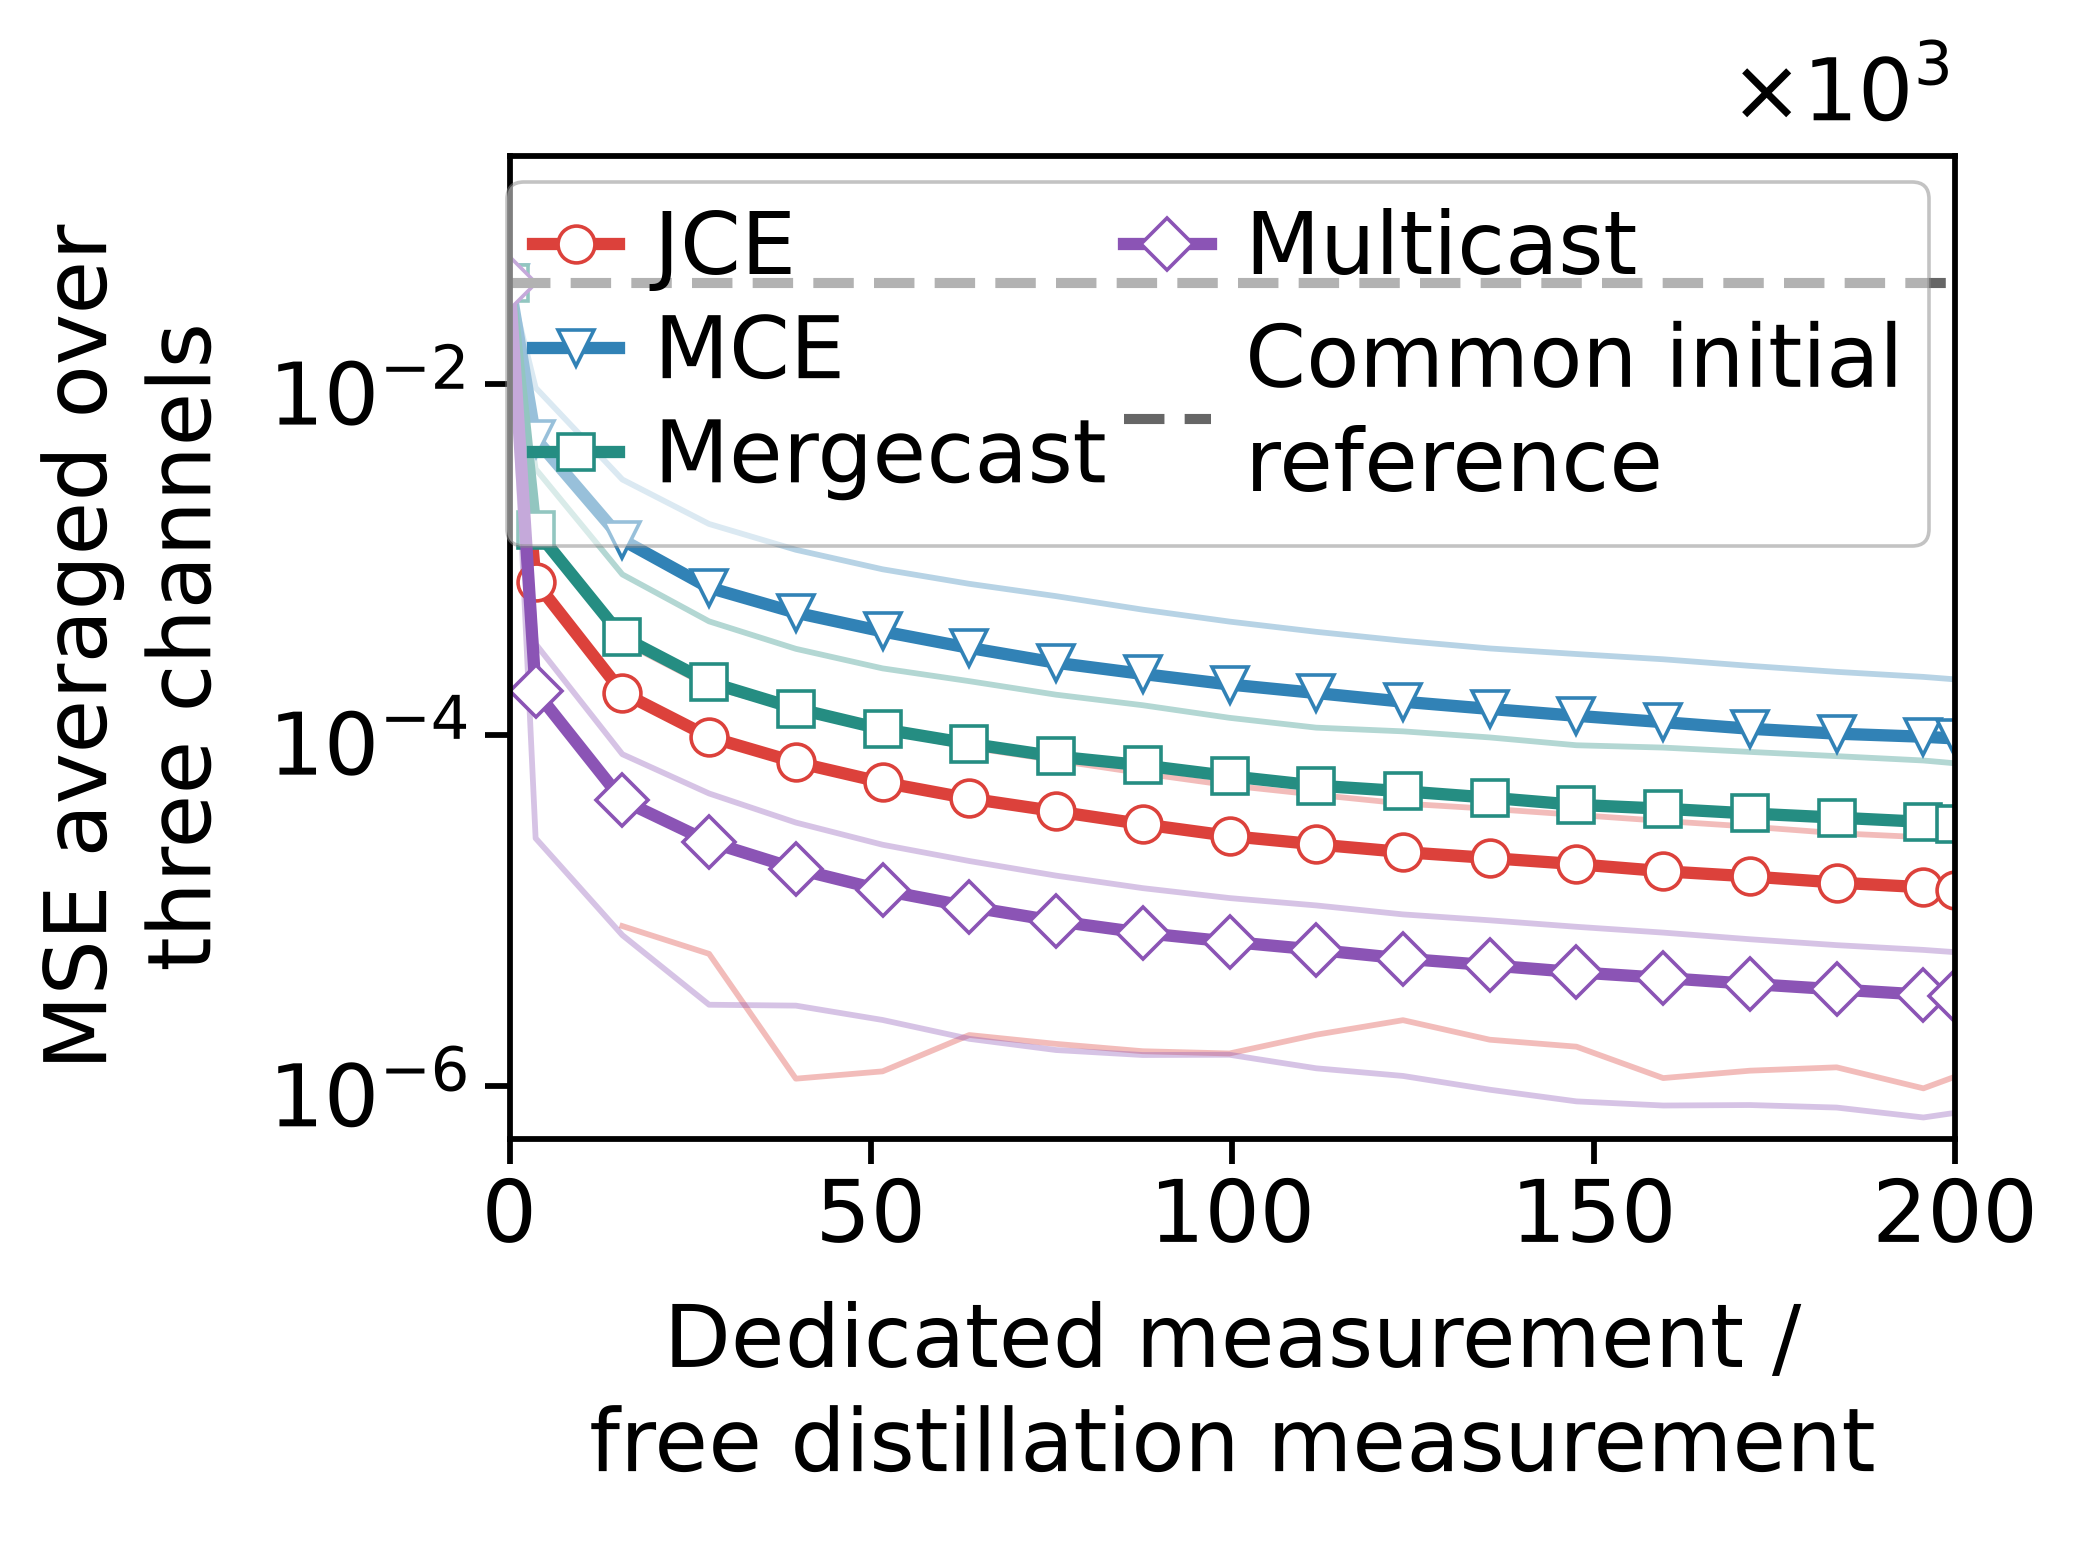
\includegraphics[width=\linewidth]
    {figures/comparison.png}
    \caption{With a depolarizing prior.}
    \label{fig:mergecast-measured-budget}
\end{subfigure}
\hfill
\begin{subfigure}[t]{0.24\textwidth}
    \centering
    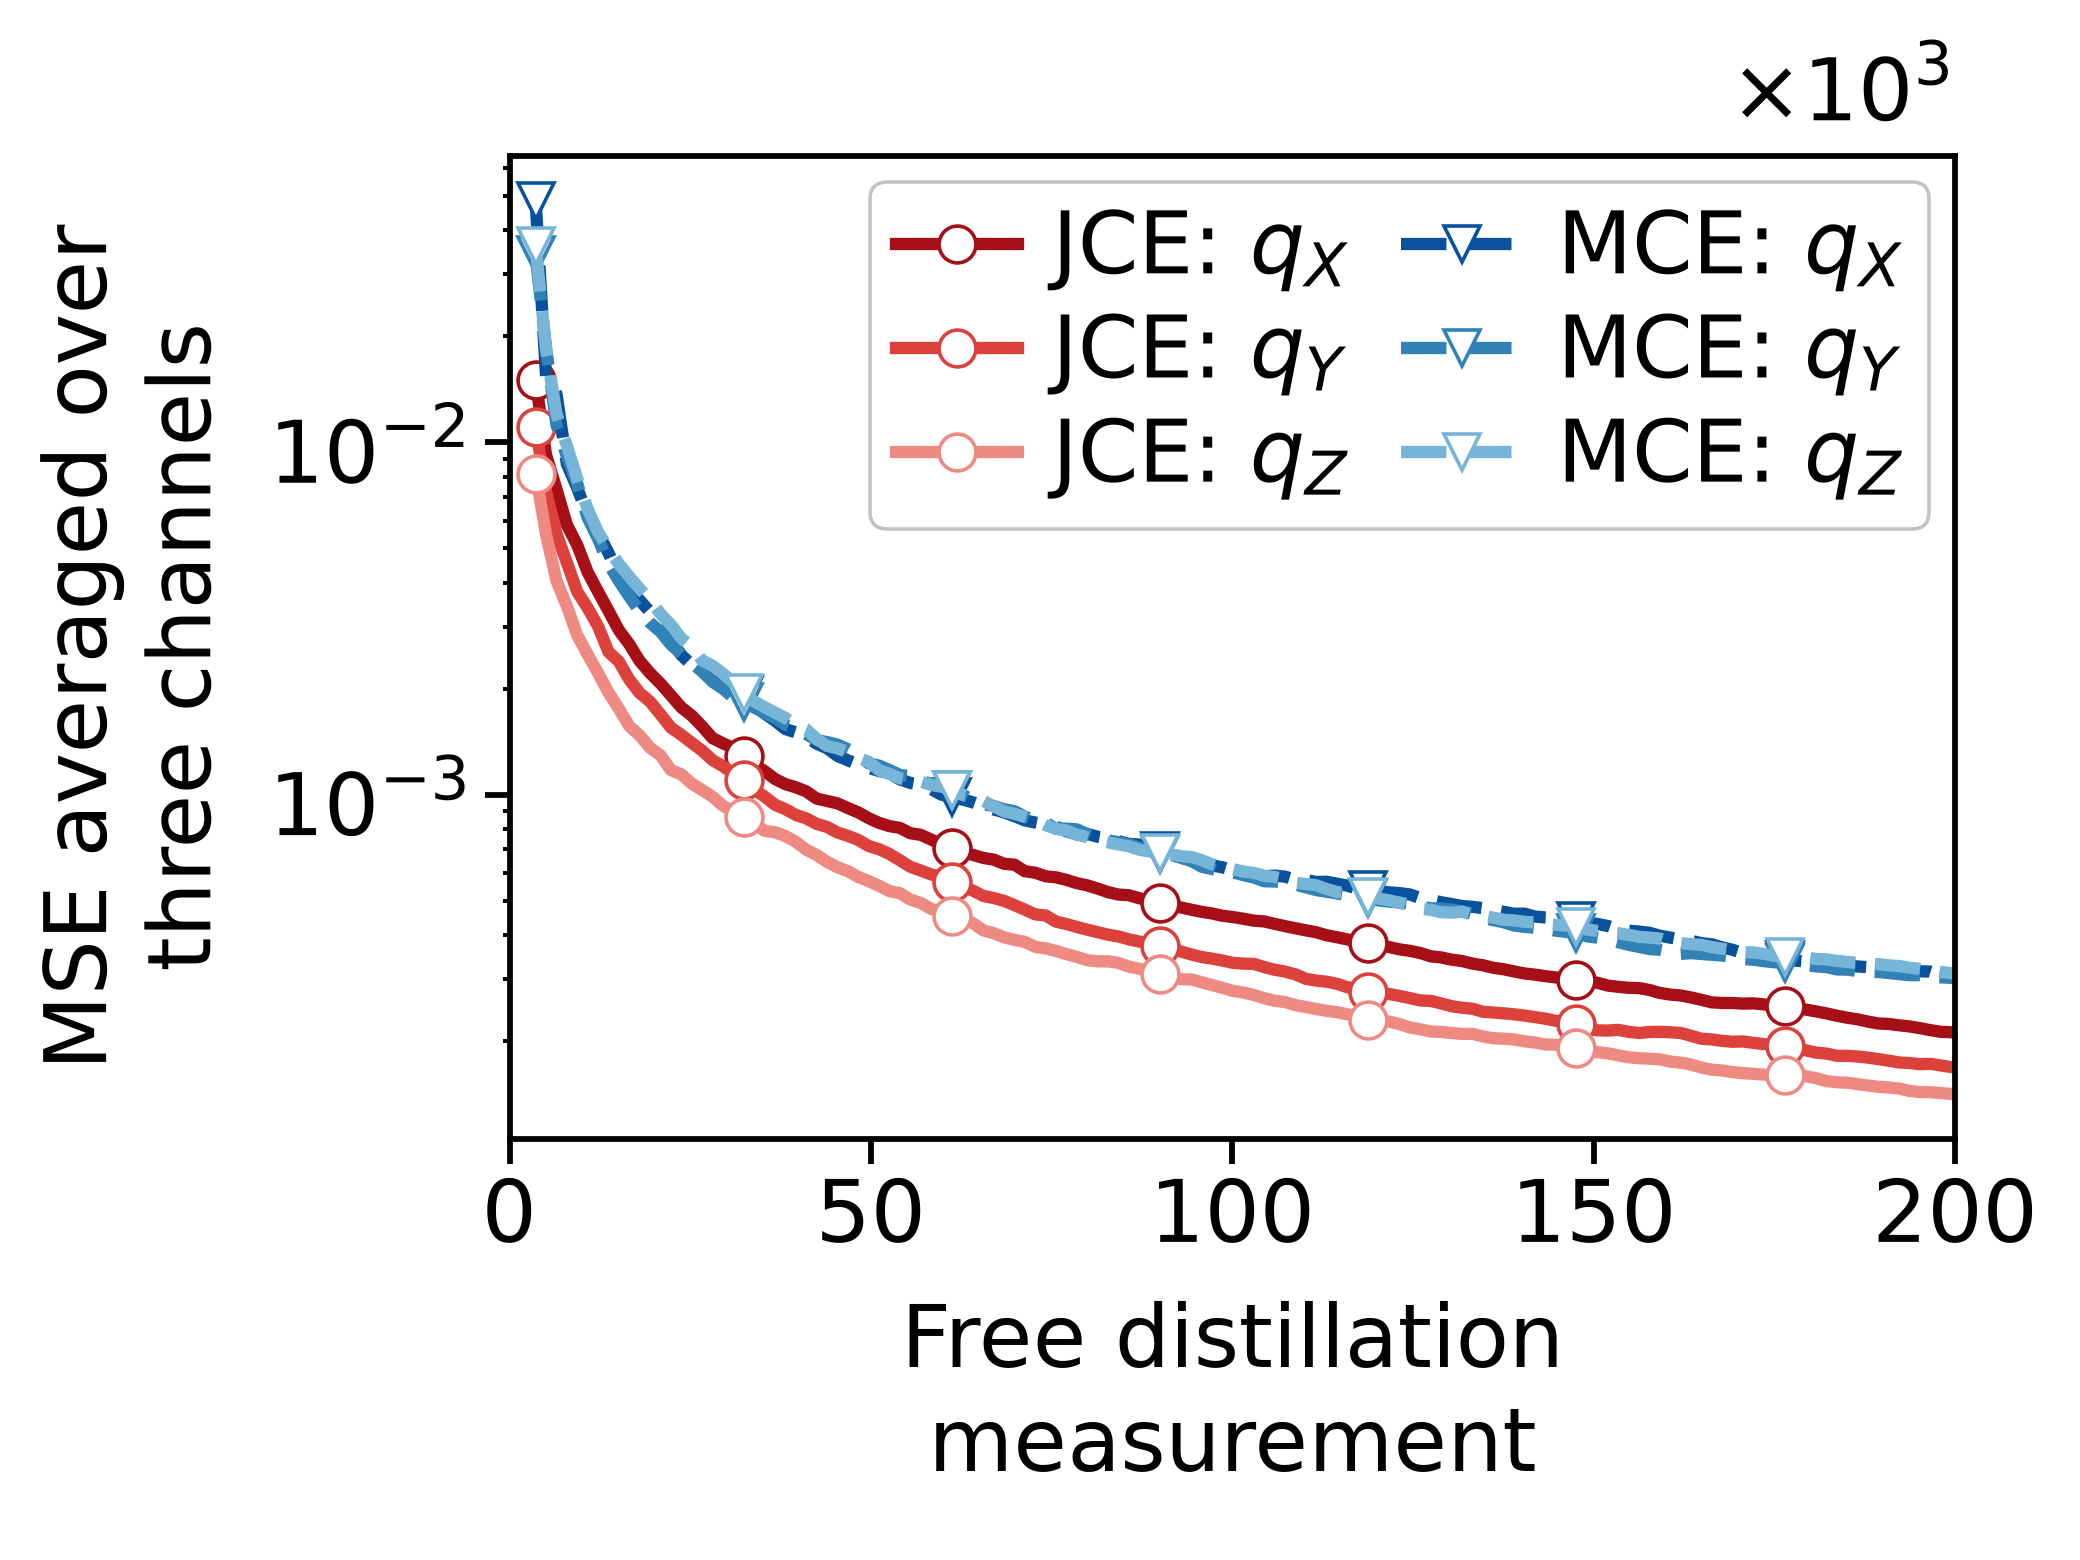
\includegraphics[width=\linewidth]
    {figures/estimator_component_mse_equal_measured_qubits.png}
    \caption{Equal round counts.}
    \label{fig:estimators-equal-rounds}
\end{subfigure}
\hfill
\begin{subfigure}[t]{0.24\textwidth}
    \centering
    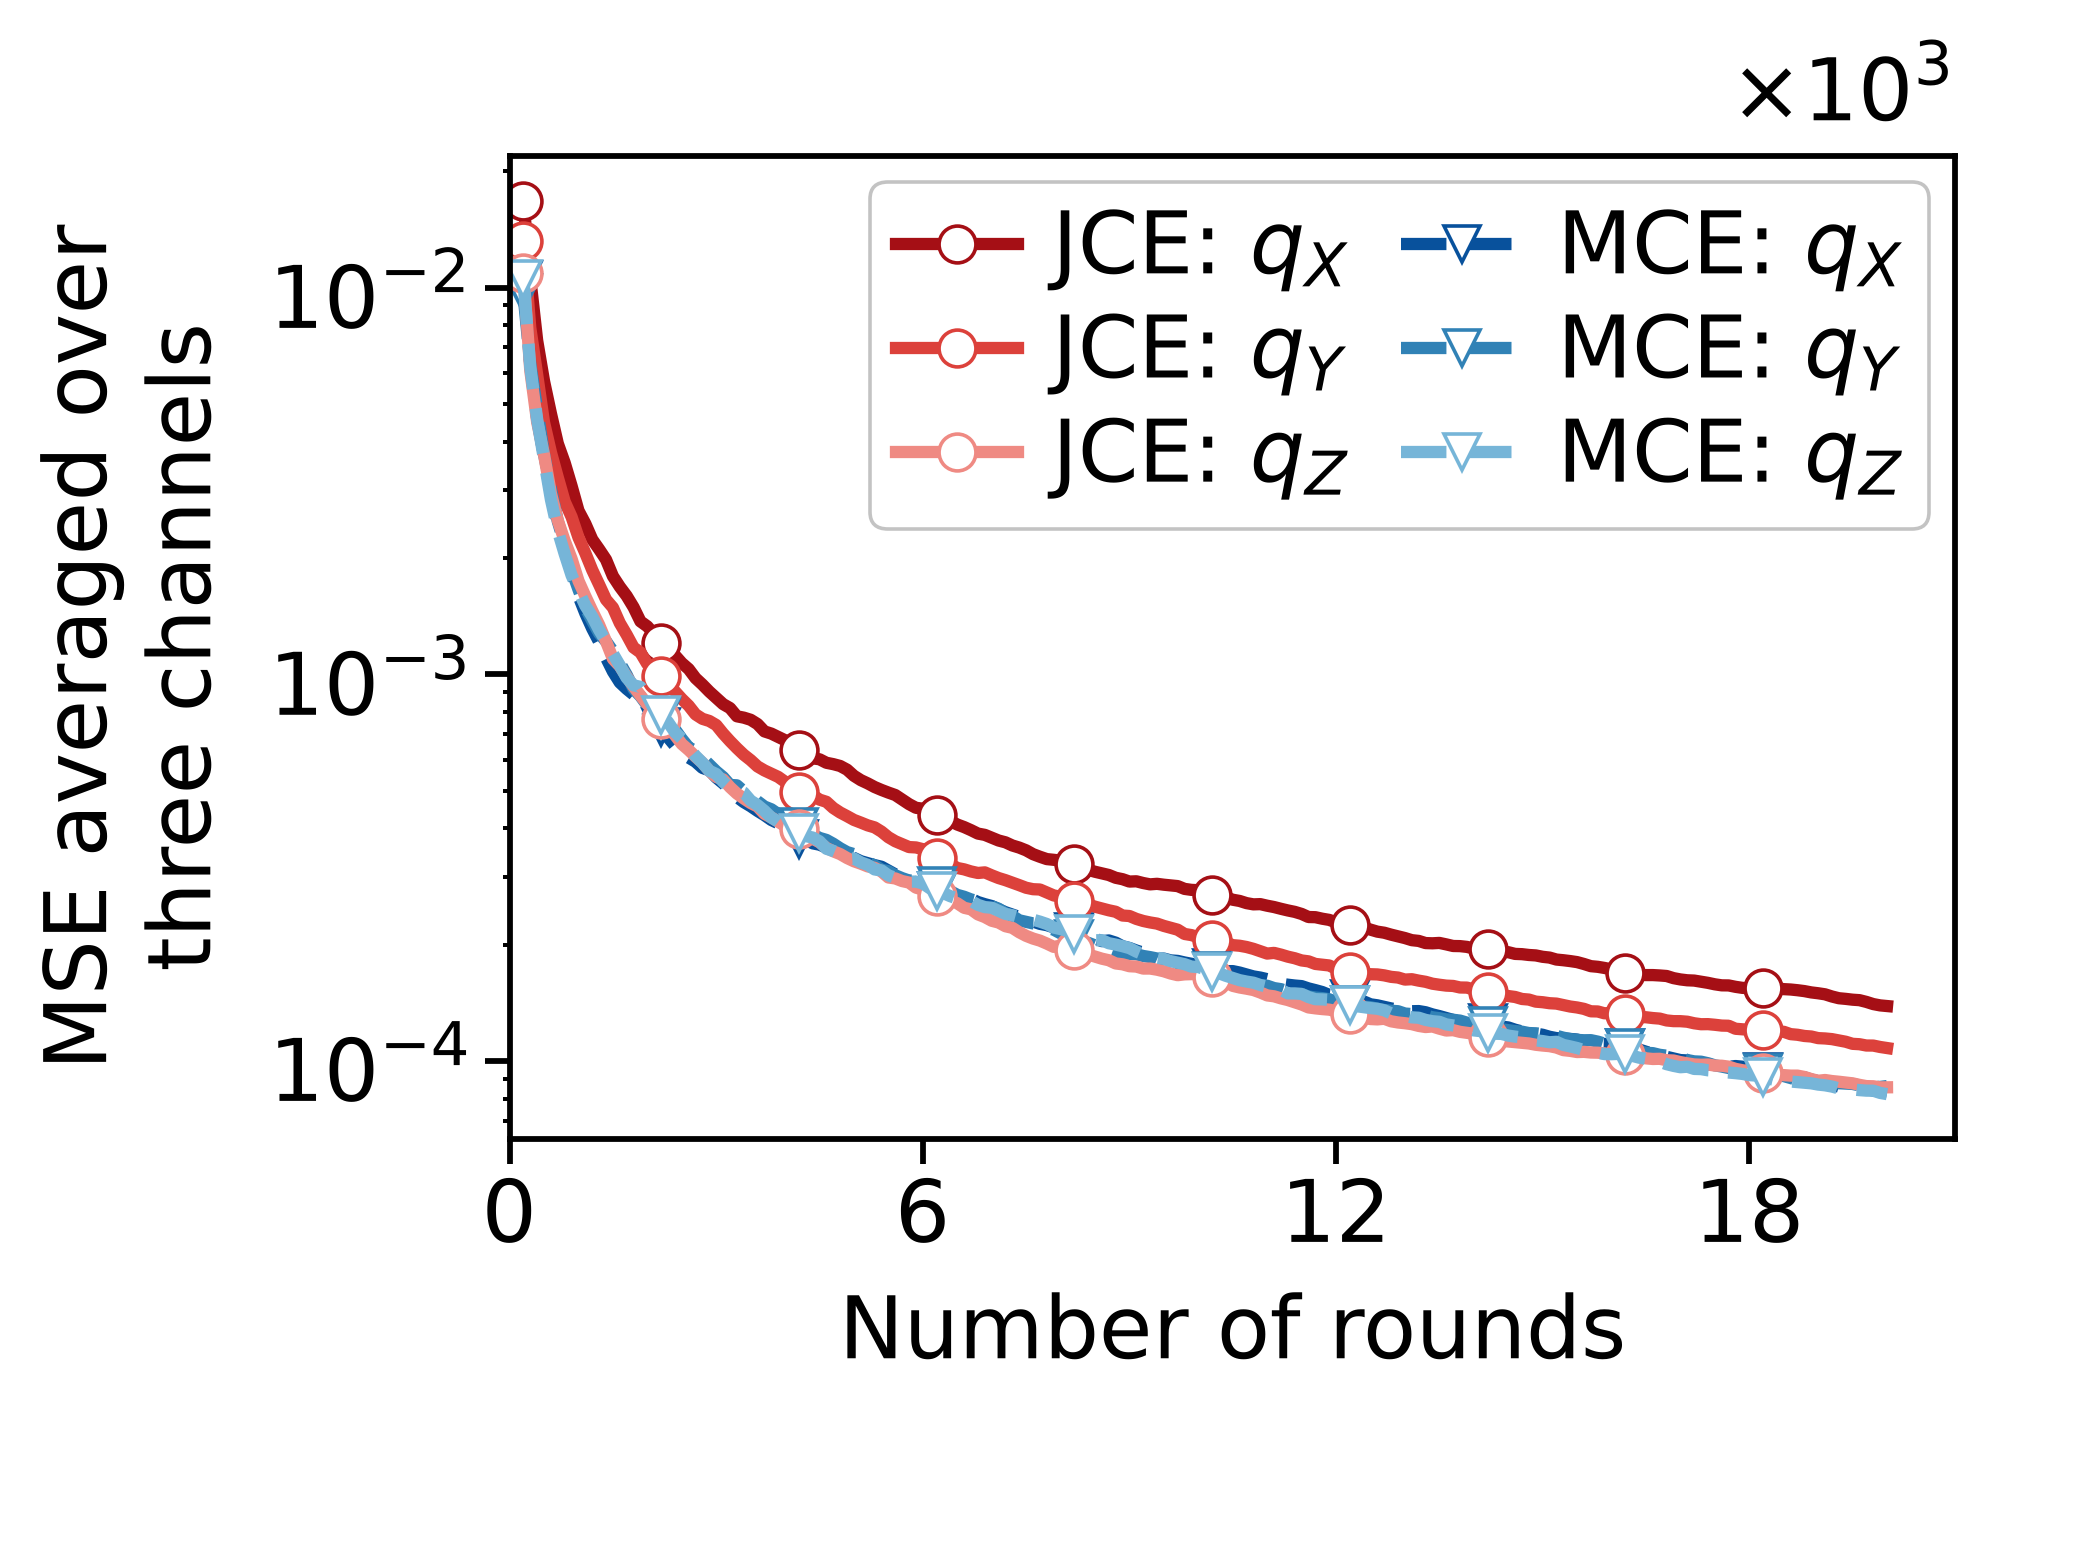
\includegraphics[width=\linewidth]
    {figures/estimator_component_mse_vs_rounds.png}
    \caption{Equal configuration counts.}
    \label{fig:estimators-equal-configurations}
\end{subfigure}

\caption{Tomography performance in the three-link star network.
(a) Comparison of JCE, MCE, and Mergecast
at equal measurement counts without a depolarizing prior,
using the MSE over nine independent Pauli parameters.
(b) Comparison with a known depolarizing model, where all methods
estimate three link parameters using maximum likelihood estimation.
Light curves in (a) and (b) indicate one standard deviation about
the mean; dashed horizontal lines mark the prescribed common
zero-data references.
(c) Component-wise MSE at equal round counts.
Each round executes four configurations for JCE
and nine for MCE.
(d) Component-wise MSE at equal numbers of configuration executions.
With $K$ executions, JCE performs $K/4$ rounds
and MCE performs $K/9$ rounds.
Component-wise errors are averaged over the three channels.
Each budget is evaluated using 1,000 Qiskit trials.}
\label{fig:star-tomography-comparisons}
\end{figure*}
\paragraph{With a depolarizing prior.}

Figure~\ref{fig:star-tomography-comparisons}(b) considers
the case in which all methods know the depolarizing structure.
Only the three parameters $(q_{P,1},q_{P,2},q_{P,3})$
are estimated, using maximum likelihood estimation.

The adapted JCE and MCE both execute three double-selection
configurations, $\rho_{12}$, $\rho_{13}$, and $\rho_{\mathrm m,23}$,
and measure 12 qubits per round.
JCE uses the joint $X/Z$ coincidence statistics, whereas
MCE uses the $Z$-coincidence marginal of the same records.
Mergecast uses two Unicast configurations and one Mergecast
configuration, measuring three qubits per round.
The Multicast baseline \cite{Andrade2024QNT} measures two
qubits per round.


Multicast achieves the lowest MSE, while JCE outperforms
Mergecast and MCE.
Because JCE and MCE use identical distillation records
in this setting, their difference demonstrates the benefit
of retaining the joint coincidence information for estimation.







% Table fragment for inclusion in the manuscript; not a standalone document.
% Requires \usepackage{booktabs} in the manuscript preamble.
% Generated from independent saved JCE/MCE records; no resampling or expected-count substitution.
% Row order: rho12, rho13, rho23_0

\subsubsection{Comparison of the two estimators}
Fig.~\ref{fig:star-tomography-comparisons}(c) and Fig.~\ref{fig:star-tomography-comparisons}(d) compare the
$X$-, $Y$-, and $Z$-component MSEs of JCE and MCE,
each averaged over the three links. Both estimators
reconstruct the channel parameters without imposing
the depolarizing constraint.

At equal measurement budgets, JCE achieves lower
component MSEs in this setting.
At equal round counts, MCE achieves lower MSEs for
the $X$ and $Y$ components, while the $Z$-component
MSEs are comparable.
For MCE, the different Pauli components are inferred
from $Z$-basis coincidence statistics under Clifford
dressing; their errors therefore depend on both the
measurement statistics and the subsequent inversion.
These comparisons use different resources: each round
of MCE executes nine configurations and measures
36 qubits, whereas each round of JCE executes four
configurations and measures 16 qubits.
Thus, equal round counts do not imply equal
measurement budgets.
The additional configurations of MCE enable estimation
without the source-state fidelity condition.
The present experiment compares their accuracy in
a regime where both estimators apply.

In addition to estimating channel parameters, both
methods retain entangled pairs with improved fidelity.
Table~\ref{tab:three-methods-mean-retained-pairs} reports
the average retained-pair counts
at an equal measurement budget.
MCE yields a slightly larger total number of
fidelity-improved pairs and more pairs in the two
higher output-fidelity groups, whereas JCE retains
more pairs in the lowest output-fidelity group.
The corresponding input and conditional output
fidelities are identical for the two methods.



\subsection{Extension to a Six-Link Triangular Network}
\label{sub2}
We next consider the network in
Fig.~\ref{fig:triangle-leaf-network}, consisting of three internal
nodes arranged in a triangle, each connected to one
peripheral monitor.
In the channel order
$(\mathcal P_1,\mathcal P_2,\mathcal P_3,
  \mathcal P_{12},\mathcal P_{13},\mathcal P_{23})$,
the true PTM parameters are
\begin{equation}
    \boldsymbol q_P
    =
    \frac{1}{75}(73,72,71,70,69,68),
    \qquad P\in\{X,Y,Z\}.
\end{equation}
Although the channels are depolarizing, reconstruction
estimates all eighteen Pauli-channel parameters independently.
\begin{figure}[tb]
\centering

% Left panel: network topology.
\begin{subfigure}[b]{0.24\textwidth}
\centering
\vspace{0pt}
\resizebox{\linewidth}{!}{%
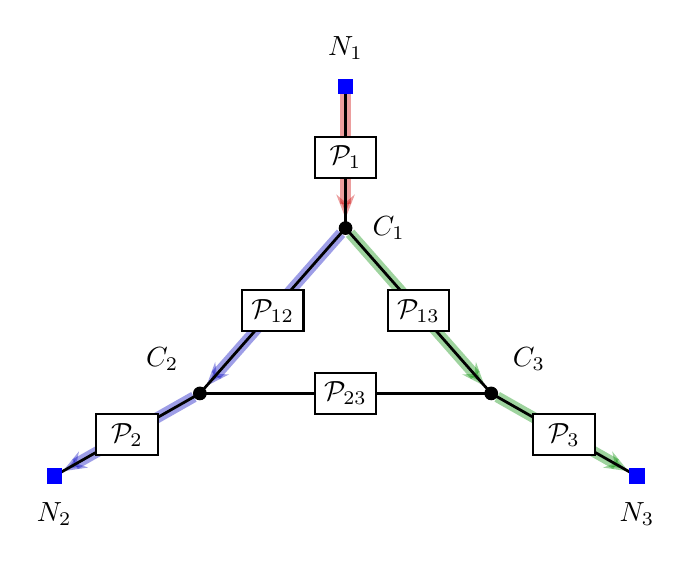
\begin{tikzpicture}[
    line/.style={draw=black,line width=1pt},
    probe/.style={
        line width=4pt,opacity=0.38,
        -{Stealth[length=3mm,width=2.3mm]},
        shorten <=2.5pt,shorten >=3.5pt
    },
    proc/.style={
        rectangle,draw=black,fill=white,thick,
        minimum width=0.78cm,minimum height=0.52cm,
        inner sep=1pt
    },
    endpoint/.style={
        rectangle,fill=blue,draw=blue,
        minimum size=0.18cm,inner sep=0pt
    },
    router/.style={
        circle,fill=black,draw=black,
        minimum size=0.16cm,inner sep=0pt
    }
]

\coordinate (C1) at (0,1.25);
\coordinate (C2) at (-1.85,-0.85);
\coordinate (C3) at (1.85,-0.85);
\coordinate (N1) at (0,3.05);
\coordinate (N2) at (-3.70,-1.90);
\coordinate (N3) at (3.70,-1.90);

\draw[probe,red!80!black] (N1)--(C1);
\draw[probe,blue!75!black] (C1)--(C2);
\draw[probe,blue!75!black] (C2)--(N2);
\draw[probe,green!55!black] (C1)--(C3);
\draw[probe,green!55!black] (C3)--(N3);

\draw[line] (N1)--(C1);
\draw[line] (C1)--(C2)--(N2);
\draw[line] (C1)--(C3)--(N3);
\draw[line] (C2)--(C3);

\node[proc] at (0,2.15) {$\mathcal P_1$};
\node[proc] at (-2.775,-1.375) {$\mathcal P_2$};
\node[proc] at (2.775,-1.375) {$\mathcal P_3$};
\node[proc] at (-0.925,0.20) {$\mathcal P_{12}$};
\node[proc] at (0.925,0.20) {$\mathcal P_{13}$};
\node[proc] at (0,-0.85) {$\mathcal P_{23}$};

\foreach \v in {C1,C2,C3}{
    \node[router] at (\v) {};
}
\node[anchor=west] at (0.22,1.25) {$C_1$};
\node[anchor=south east] at (-2.00,-0.68) {$C_2$};
\node[anchor=south west] at (2.00,-0.68) {$C_3$};

\foreach \v in {N1,N2,N3}{
    \node[endpoint] at (\v) {};
}
\node[above=6pt] at (N1) {$N_1$};
\node[below=6pt] at (N2) {$N_2$};
\node[below=6pt] at (N3) {$N_3$};

\end{tikzpicture}%
}
\caption{Six-link triangular network.}
\label{fig:triangle-leaf-network}
\end{subfigure}
\hfill
% Right panel: estimation error.
\begin{subfigure}[b]{0.24\textwidth}
\centering
\vspace{0pt}
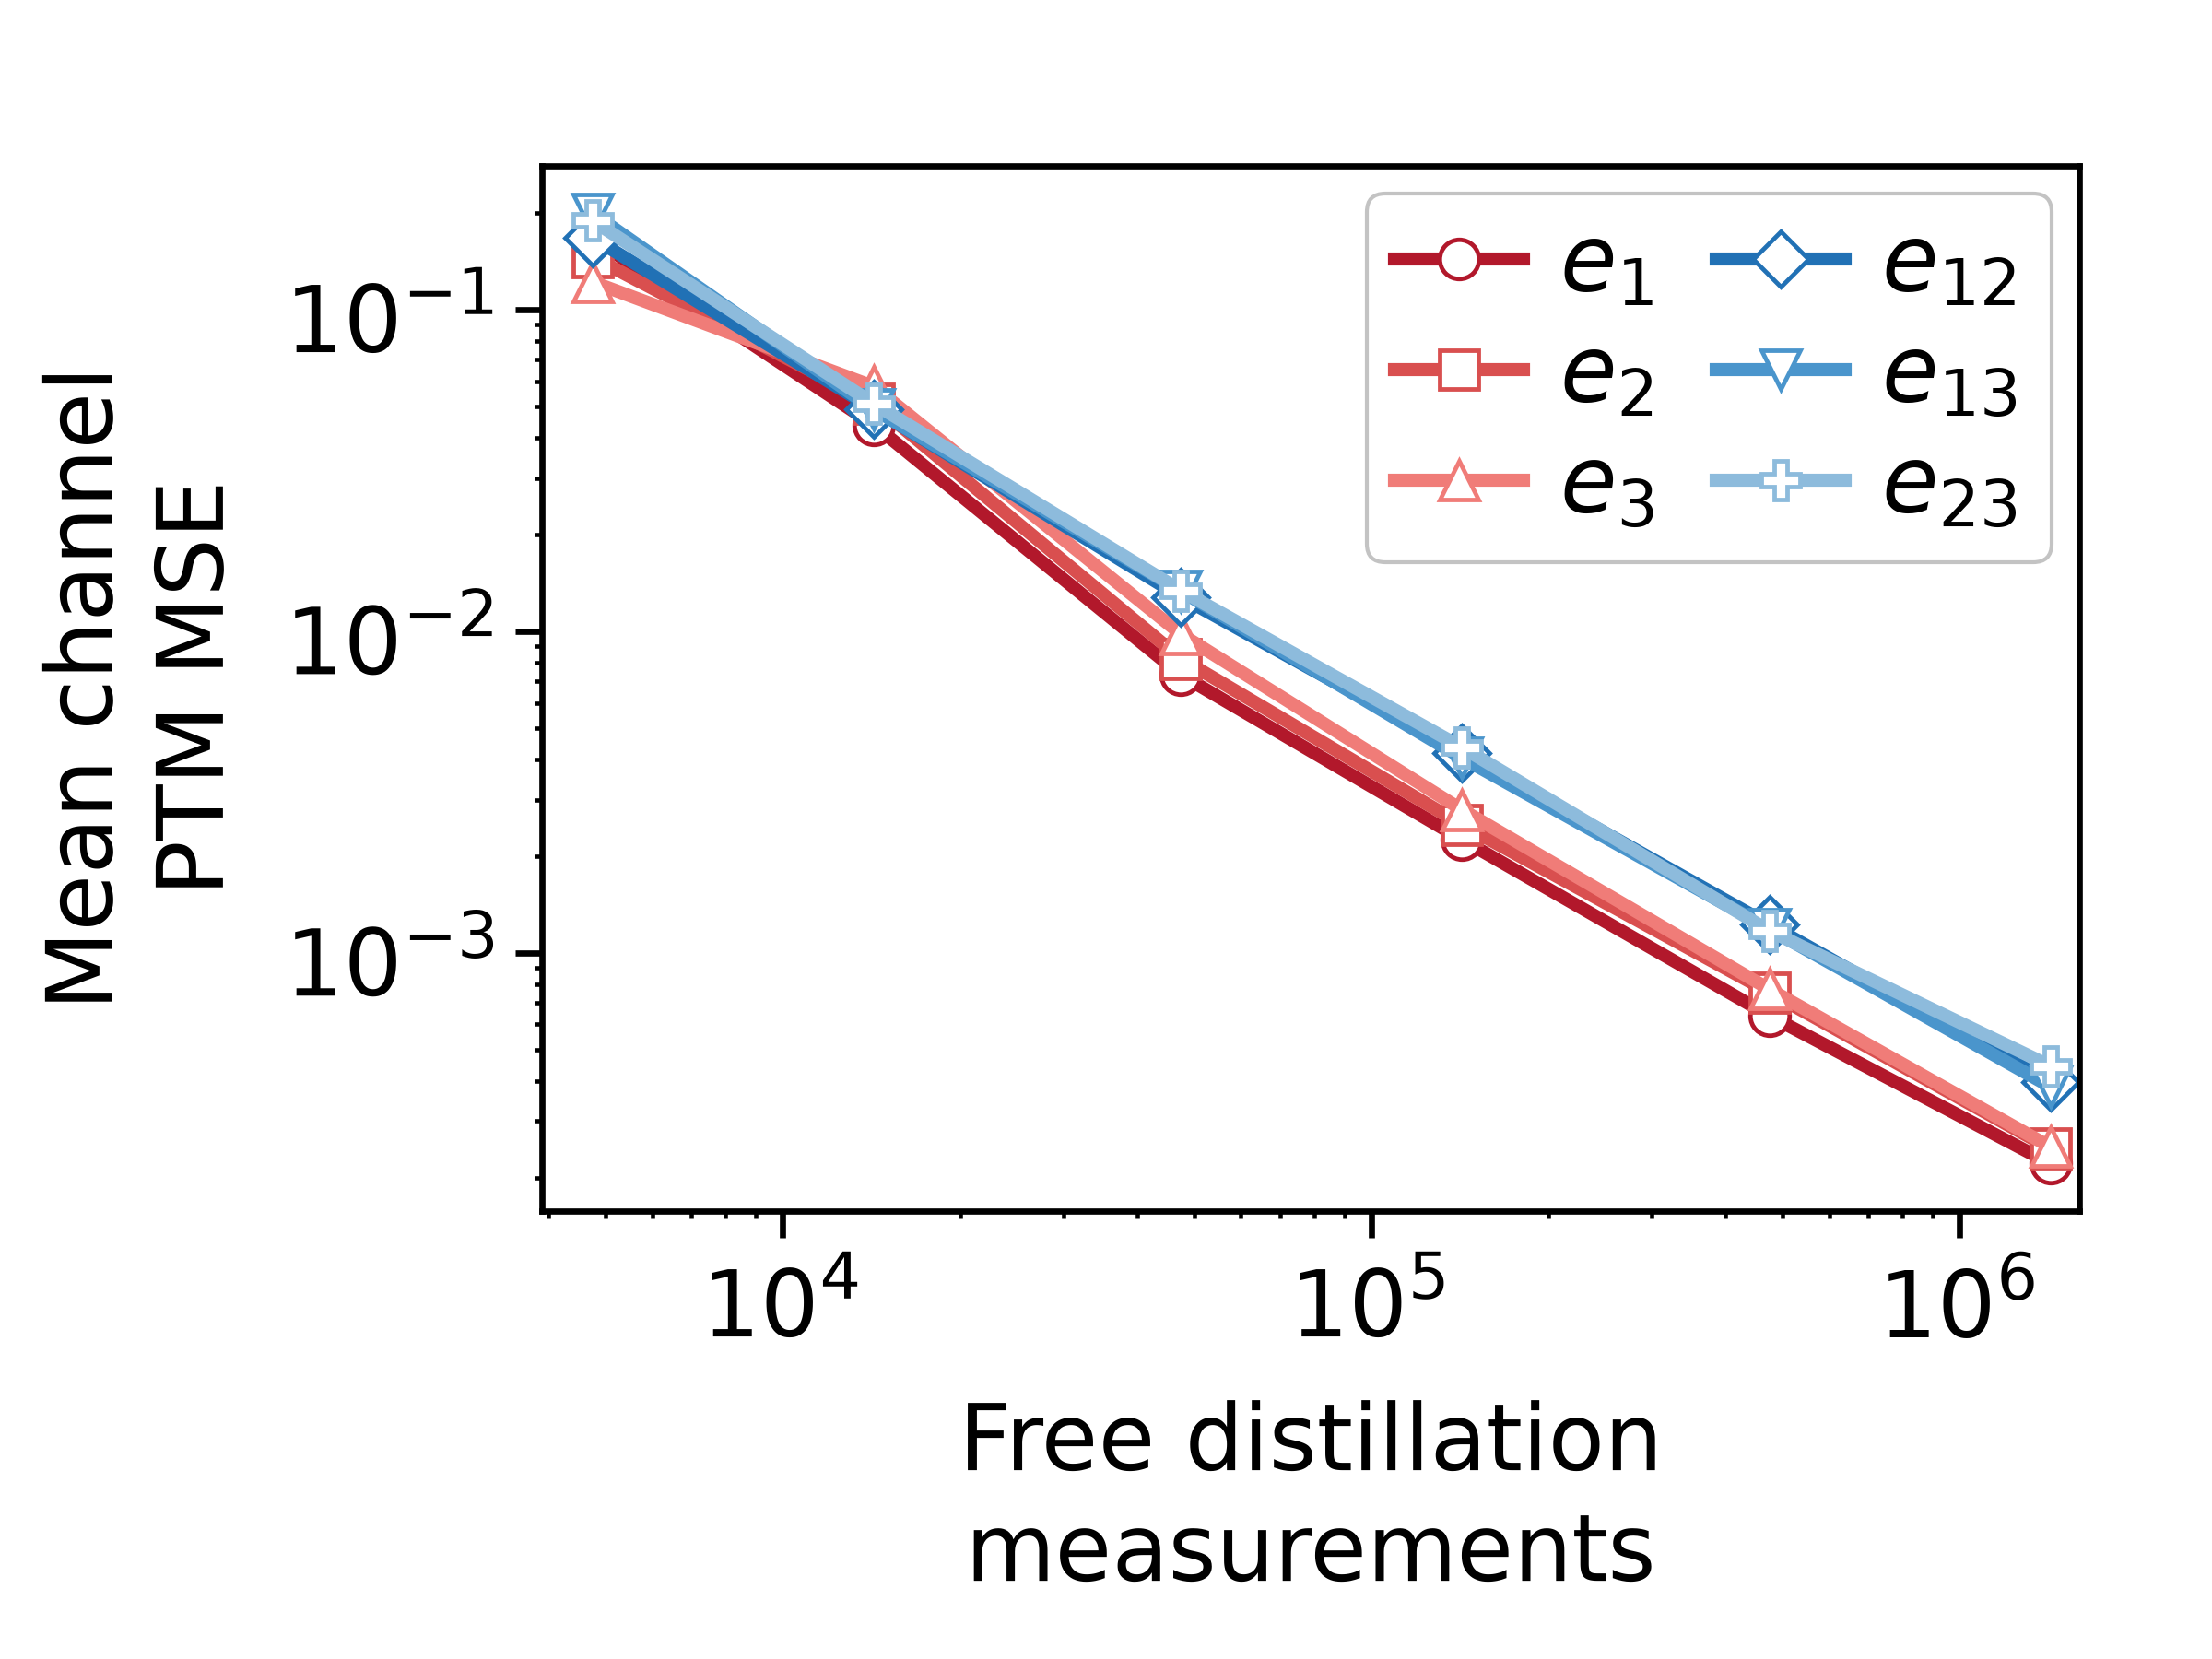
\includegraphics[width=\linewidth]{figures/triangle_sixlink.png}
\caption{Mean per-channel PTM MSE.}
\label{fig:triangle-edge-mse}
\end{subfigure}

\caption{Network topology and tomography performance in a six-link
triangular network.
(a) Peripheral monitors $N_1,N_2,N_3$ connect to internal nodes
$C_1,C_2,C_3$. Colored arrows illustrate an effective star centered
at $C_1$, with channels $\mathcal P_1$,
$\mathcal P_2\circ\mathcal P_{12}$, and
$\mathcal P_3\circ\mathcal P_{13}$.
Analogous constructions at $C_2$ and $C_3$ provide the observations
used for the two-stage reconstruction.
(b) Mean PTM MSE versus the number of distillation measurements
reused for tomography. Red curves represent the outer channels
$e_1,e_2,e_3$, and blue curves represent the inner channels
$e_{12},e_{13},e_{23}$.}
\label{fig:triangle-network-results}
\end{figure}
We apply JCE to three effective stars centered at
$C_1$, $C_2$, and $C_3$.
For example, the star centered at $C_1$ has effective
channels $\mathcal P_1$, $\mathcal P_2\circ\mathcal P_{12}$,
and $\mathcal P_3\circ\mathcal P_{13}$.
For each effective star, we perform two unicast
double-selection configurations and two modified
Mergecast double-selection configurations, with and
without Clifford dressing.
In the first stage, we estimate the outer channels
and the composite branches.
In the second stage, we recover the internal-channel
parameters by dividing the estimated composite-branch
PTM parameters by the corresponding outer-channel
estimates.
Consequently, estimation errors in the outer channels
also propagate into the internal-channel estimates.

Fig.~\ref{fig:triangle-edge-mse} reports the MSE of
each channel, averaged over its three Pauli components
and the algebraically valid repetitions.
The horizontal axis counts the measurements performed
during distillation and reused for tomography,
denoted as \emph{free distillation measurements}.
One complete round across the three effective stars
executes twelve configurations and measures
48 qubits.

The MSE decreases overall for all six channels as the
measurement budget increases.
In this setting, the outer channels exhibit lower
MSE than the internal channels, consistent with
the additional error propagation introduced by
the second reconstruction stage.
These results demonstrate the applicability of
the proposed reconstruction procedure to a network
beyond the three-link star topology.











\section{Conclusion}

In this work, we presented a distillation-assisted framework for quantum
network tomography that uses the same measurement records to characterize
internal links and support entanglement distillation. For a three-link
star network with unknown Pauli channels, we combined \unicast{} and
\mergecast{} preparations with Clifford dressing to develop two estimators
that recover link-level channel parameters without additional tomography
measurements.
The \jce{} exploits marginal and joint coincidence statistics to improve
estimation accuracy under a source-state fidelity condition, while the
\mce{} removes this requirement through uniform Clifford dressing at the
cost of additional configurations. The two estimators therefore offer
a trade-off between measurement requirements and applicability.

Qiskit simulations demonstrated that both estimators accurately
reconstruct link channels while retaining entangled pairs with improved
fidelity in the tested regime. We further extended the framework to a
six-link triangular network, demonstrating its applicability beyond
the basic star topology.
Future work will extend the framework to account for state preparation
and measurement (SPAM) errors and explore its application to more general
network topologies. We also plan to develop distillation protocols that
improve both tomography accuracy and the fidelity of the retained
entangled pairs. These results establish distillation-assisted tomography as a promising
approach to simultaneous channel characterization and high-fidelity
entanglement distribution.
\appendices
% \xw{defer to some place later or appendix or discussion.}
For each Pauli component, knowing the sign of one link parameter
would resolve the ambiguity, since the other two signs follow from
the measured products. In particular, a known reference link
\(i_0\) satisfying \(A_{i_0}>1/2\) would imply
\(q_{X,\ell _0},q_{Y,\ell _0},q_{Z,\ell _0}>0\), allowing all three channels
to be identified from the three sets of pairwise products.
In this work, we do not assume such prior knowledge. 

\section{Proof of Lemma~\ref{lem:double-selection-statistics}}
\label{app:double-selection}

We label the Bell states by two bits \(a,b\in\{0,1\}\):
\begin{equation}
\ket{\beta_{ab}}
:=
(I\otimes X^aZ^b)\ket{\Phi^+}.
\end{equation}
The labels \((0,0),(1,0),(1,1),(0,1)\) correspond to
\(\ket{\Phi^+},\ket{\Psi^+},\ket{\Psi^-},\ket{\Phi^-}\),
respectively.

Let \((a_i,b_i)\) denote the Bell label of the \(i\)th input pair.
After the bilateral CNOTs from pair \(1\) to pair \(2\) and from
pair \(3\) to pair \(2\), the output labels are
\begin{equation}
\begin{aligned}
(a_1',b_1')
&=(a_1,\;b_1\oplus b_2),\\
(a_2',b_2')
&=(a_1\oplus a_2\oplus a_3,\;b_2),\\
(a_3',b_3')
&=(a_3,\;b_2\oplus b_3).
\end{aligned}
\label{eq:double-selection-bell-labels}
\end{equation}
Thus, coincidence in the \(Z\) measurements occurs if and only if
\(a_1\oplus a_2\oplus a_3=0\), while coincidence in the \(X\)
measurements occurs if and only if \(b_2\oplus b_3=0\).

Define
\begin{equation}
\begin{aligned}
x&:=\mathbb E[(-1)^b]=2(q_1+q_2)-1,\\
y&:=\mathbb E[(-1)^{a+b}]=2(q_1+q_3)-1,\\
z&:=\mathbb E[(-1)^a]=2(q_1+q_4)-1.
\end{aligned}
\label{eq:double-selection-correlations}
\end{equation}
Let
\[
U:=(-1)^{a_1+a_2+a_3},
\qquad
V:=(-1)^{b_2+b_3}.
\]
By independence of the three input pairs,
\begin{equation}
\mathbb E[U]=z^3,
\qquad
\mathbb E[V]=x^2,
\qquad
\mathbb E[UV]=zy^2.
\end{equation}
The coincidence probabilities therefore satisfy
\begin{equation}
\begin{aligned}
p_Z
&:=
\Pr(z_A=z_B)
=
\mathbb E\left[\frac{1+U}{2}\right]
=
\frac{1+z^3}{2},\\
p_X
&:=
\Pr(x_A=x_B)
=
\mathbb E\left[\frac{1+V}{2}\right]
=
\frac{1+x^2}{2},\\
p_{XZ}
&:=
\Pr(z_A=z_B,\;x_A=x_B)\\
&=
\mathbb E\left[\frac{(1+U)(1+V)}{4}\right]
=
\frac{1+z^3+x^2+zy^2}{4}.
\end{aligned}
\label{eq:double-selection-probabilities}
\end{equation}

Since \(q_1>1/2\), all three quantities \(x,y,z\) are strictly
positive. Hence, these relations can be uniquely inverted:
\begin{equation}
\begin{aligned}
x&=\sqrt{2p_X-1},\\
z&=\sqrt[3]{2p_Z-1},\\
y&=
\sqrt{
\frac{4p_{XZ}-2p_X-2p_Z+1}{z}
}.
\end{aligned}
\label{eq:double-selection-inversion}
\end{equation}
The positive square-root branches are fixed by the assumption
\(q_1>1/2\), which also ensures \(z>0\).
The Bell-state probabilities are then recovered as
\begin{equation}
\begin{bmatrix}
q_1\\q_2\\q_3\\q_4
\end{bmatrix}
=
\frac{1}{4}
\begin{bmatrix}
1+x+y+z\\
1+x-y-z\\
1-x+y-z\\
1-x-y+z
\end{bmatrix}.
\label{eq:double-selection-state-reconstruction}
\end{equation}
This proves that the three coincidence probabilities uniquely
determine the input Bell-diagonal state.

It remains to determine the conditional output fidelity.
By Eq.~\eqref{eq:double-selection-bell-labels}, the first output
pair is in \(\ket{\Phi^+}\) when
\[
a_1=0,
\qquad
b_1=b_2.
\]
Combining these conditions with the acceptance conditions gives
\[
a_2=a_3,
\qquad
b_1=b_2=b_3.
\]
Therefore, the unnormalized weight of \(\ket{\Phi^+}\) in the
accepted output is
\begin{equation}
\begin{aligned}
N_{\Phi^+}
&=
q_1(q_1^2+q_2^2)+q_4(q_4^2+q_3^2)\\
&=
q_1^3+q_4^3+q_1q_2^2+q_4q_3^2.
\end{aligned}
\end{equation}
Since \(p_{XZ}\geq q_1^3>0\), normalization yields
\begin{equation}
\begin{aligned}
F_{\mathrm{out}}
&=
\frac{N_{\Phi^+}}{p_{XZ}}\\
&=
\frac{
4\left(q_1^3+q_4^3+q_1q_2^2+q_4q_3^2\right)
}{
1+z^3+x^2+zy^2
},
\end{aligned}
\end{equation}
which establishes
Eq.~\eqref{eq:double-selection-output-fidelity}.
\section{Details for Modified \mergecast in Figure \ref{fig:modified-mergecast}}
Below, we present the quantum states at slices \(1\)--\(4\) of
Fig.~\ref{fig:modified-mergecast}. Let \(R\) denote the qubit retained
by \(A_1\), \(T\) the transmitted half of the Bell pair, and \(A\) the
auxiliary qubit sent by \(A_2\). We use the tensor-product ordering
\((R,T,A)\). Since the corresponding three-qubit Pauli--Liouville
vectors contain \(64\) entries, we list only the potentially nonzero
components with respect to the ordered sparse basis
\begin{equation}
\mathcal B_3:=
\left(
III,IIZ,XXI,XXZ,YYI,YYZ,ZZI,ZZZ
\right),
\end{equation}
where, for example, \(XXZ:=X_R\otimes X_T\otimes Z_A\).

At slice \(1\), the joint state is
\begin{equation}
\rho_{RTA}^{(1)}
=
\ket{\Phi^+}\!\bra{\Phi^+}_{RT}
\otimes
\ket{0}\!\bra{0}_A,
\end{equation}
whose nonzero Pauli--Liouville components are
\begin{equation}
\left.\left|\rho_{RTA}^{(1)}\right\rangle\right\rangle_{\mathcal B_3}
=
\begin{bmatrix}
1\\
1\\
1\\
1\\
-1\\
-1\\
1\\
1
\end{bmatrix}.
\end{equation}

After \(T\) and \(A\) pass through \(\mathcal P_1\) and
\(\mathcal P_2\), respectively, the state at slice \(2\) is
\begin{equation}
\rho_{RTA}^{(2)}
=
\left(
\mathcal I_R\otimes\mathcal P_1\otimes\mathcal P_2
\right)
\left(\rho_{RTA}^{(1)}\right),
\end{equation}
with
\begin{equation}
\left.\left|\rho_{RTA}^{(2)}\right\rangle\right\rangle_{\mathcal B_3}
=
\begin{bmatrix}
1\\
q_{Z2}\\
q_{X1}\\
q_{X1}q_{Z2}\\
-q_{Y1}\\
-q_{Y1}q_{Z2}\\
q_{Z1}\\
q_{Z1}q_{Z2}
\end{bmatrix}.
\end{equation}

Node \(C\) then applies
\(U_{\mathrm C}:=\operatorname{CNOT}_{A\rightarrow T}\).
Immediately after the CNOT, the state is
\begin{equation}
\widetilde{\rho}_{RTA}^{(3)}
=
U_{\mathrm C}\rho_{RTA}^{(2)}U_{\mathrm C}^{\dagger},
\end{equation}
and its nonzero components are
\begin{equation}
\left.\left|\widetilde{\rho}_{RTA}^{(3)}
\right\rangle\right\rangle_{\mathcal B_3}
=
\begin{bmatrix}
1\\
q_{Z2}\\
q_{X1}\\
q_{X1}q_{Z2}\\
-q_{Y1}q_{Z2}\\
-q_{Y1}\\
q_{Z1}q_{Z2}\\
q_{Z1}
\end{bmatrix}.
\end{equation}
Here, the CNOT exchanges the Pauli components
\[
YYI\longleftrightarrow YYZ,
\qquad
ZZI\longleftrightarrow ZZZ,
\]
while leaving the other components in \(\mathcal B_3\) unchanged.

Tracing out the auxiliary qubit removes all Pauli strings whose
auxiliary component is \(Z\). Therefore, at slice \(3\),
\begin{equation}
\rho_{RT}^{(3)}
:=
\operatorname{Tr}_A
\left(\widetilde{\rho}_{RTA}^{(3)}\right)
\end{equation}
has the restricted Pauli--Liouville representation
\begin{equation}
\left.\left|\rho_{RT}^{(3)}\right\rangle\right\rangle
=
\begin{bmatrix}
1\\
q_{X1}\\
-q_{Y1}q_{Z2}\\
q_{Z1}q_{Z2}
\end{bmatrix},
\end{equation}
with respect to the ordered basis
\((II,XX,YY,ZZ)\).

Finally, after \(T\) passes through \(\mathcal P_3\), the state shared
between \(A_1\) and \(A_3\) at slice \(4\) is
\begin{equation}
\rho_{13}^{(0)}
=
\left(\mathcal I_R\otimes\mathcal P_3\right)
\left(\rho_{RT}^{(3)}\right),
\end{equation}
and hence
\begin{equation}
\left.\left|\rho_{13}^{(0)}\right\rangle\right\rangle
=
\begin{bmatrix}
1\\
q_{X1}q_{X3}\\
-q_{Y1}q_{Z2}q_{Y3}\\
q_{Z1}q_{Z2}q_{Z3}
\end{bmatrix}.
\label{eq:mergecast-slice-state}
\end{equation}
\bibliographystyle{IEEEtran}
\bibliography{ref}

\end{document}
